% ------------------------ Appendix ------------------------ 


\begin{appendix}

\begin{center}
{\Large\bf Supplementary: Reproducible scaling laws for contrastive language-image learning}
\end{center}

\section{Further details on distributed training}
\label{appendix:distributed_training}

% Details in distributed training - amount of GPUs, time spent, scaling plots

%\subsection{JUWELS Booster Supercomputer}
\subsection{Supercomputer specifications}
\label{appendix:booster}

The JUWELS Booster~\citep{JUWELSBooster2020} supercomputer used for training  consists of \num{936} compute nodes that host four NVIDIA A100 GPUs each, providing \num{3744}~GPUs in total. The installed A100 Tensor Core GPUs~(\SI{40}{\giga\byte}) provide \SI{19.5}{\tera\floppersec} of $\text{FP64}_\text{TC}$ computing performance each. The GPUs are hosted by AMD EPYC 7402 CPUs with $2\times 24$~cores (SMT-2) per node, clocked with \SI{2.8}{\giga\Hz}. Each node is diskless and is equipped with \SI{512}{\giga\byte} of RAM. The network is based on Mellanox HDR200 InfiniBand, with four Mellanox ConnectX~6 devices per node, each providing \SI{200}{\giga\bit\per\second} bandwidth per direction.

% remove for the submission ~\citep{JUWELSBooster2020}, re-introduce in final version

% Installed in November 2020, JUWELS Booster~\citep{JUWELSBooster2020} features \num{936} compute nodes that host four NVIDIA A100 GPUs each, providing \num{3744}~GPUs in total. The installed A100 Tensor Core GPUs~(\SI{40}{\giga\byte}) provide \SI{19.5}{\tera\floppersec} of $\text{FP64}_\text{TC}$ computing performance each. The GPUs are hosted by AMD EPYC 7402 CPUs with $2\times 24$~cores (SMT-2) per node, clocked with \SI{2.8}{\giga\Hz}. Each node is diskless and is equipped with \SI{512}{\giga\byte} of RAM. The network of JUWELS Booster is based on Mellanox HDR200 InfiniBand, with four Mellanox ConnectX~6 devices per node, each providing \SI{200}{\giga\bit\per\second} bandwidth per direction.

The NVIDIA A100 GPUs reach peak efficiency of \SI{48,75}{\giga\floppersec\per\watt} when utilizing the $\text{FP64}$ Tensor Cores. This made the employed machine rank highest in the Green500 list as of November 2020 as the most energy efficient supercomputer among the first 100 machines of the Top500 list with \SI{25}{\giga\floppersec\per\watt}.

% The NVIDIA A100 GPUs installed into JUWELS Booster reach peak efficiency of \SI{48,75}{\giga\floppersec\per\watt} when utilizing the $\text{FP64}$ Tensor Cores. This made JUWELS Booster rank highest in the Green500 list as of November 2020 as the most energy efficient supercomputer among the first 100 machines of the Top500 list with \SI{25}{\giga\floppersec\per\watt}.

%\subsection{JUWELS Booster Energy Efficiency}

\subsection{Scaling and training time}
\label{appendix:scaling}

Here, we report scaling behavior during large-scale pre-training  using ViT-L/14 as a vision backbone with OpenCLIP \citep{ilharco_gabriel_2021_5143773}.
We performed scaling experiments to assess the scalability of data parallel training distributed across many GPUs on multiple nodes using PyTorch DDP.
The efficiency in Figure \ref{fig:speedup_clip} is computed using the following formula: $E(N) = 100 \times \frac{T(N)}{N \times T(1)}$. $T(N)$ is the total measured throughput in Im/s for $N$ GPUs. The best achievable efficiency, when scaling is perfect, is 100\%.We observe that scaling is sufficiently close to ideal linear, staying above $\approx 84\%$ for 1024 GPUs (256 nodes).
We also provide the raw throughput (Im/s) numbers in Figure \ref{fig:throughput_clip}. 
    
\begin{figure}[ht]
\begin{subfigure}{.5\textwidth}
  \centering
  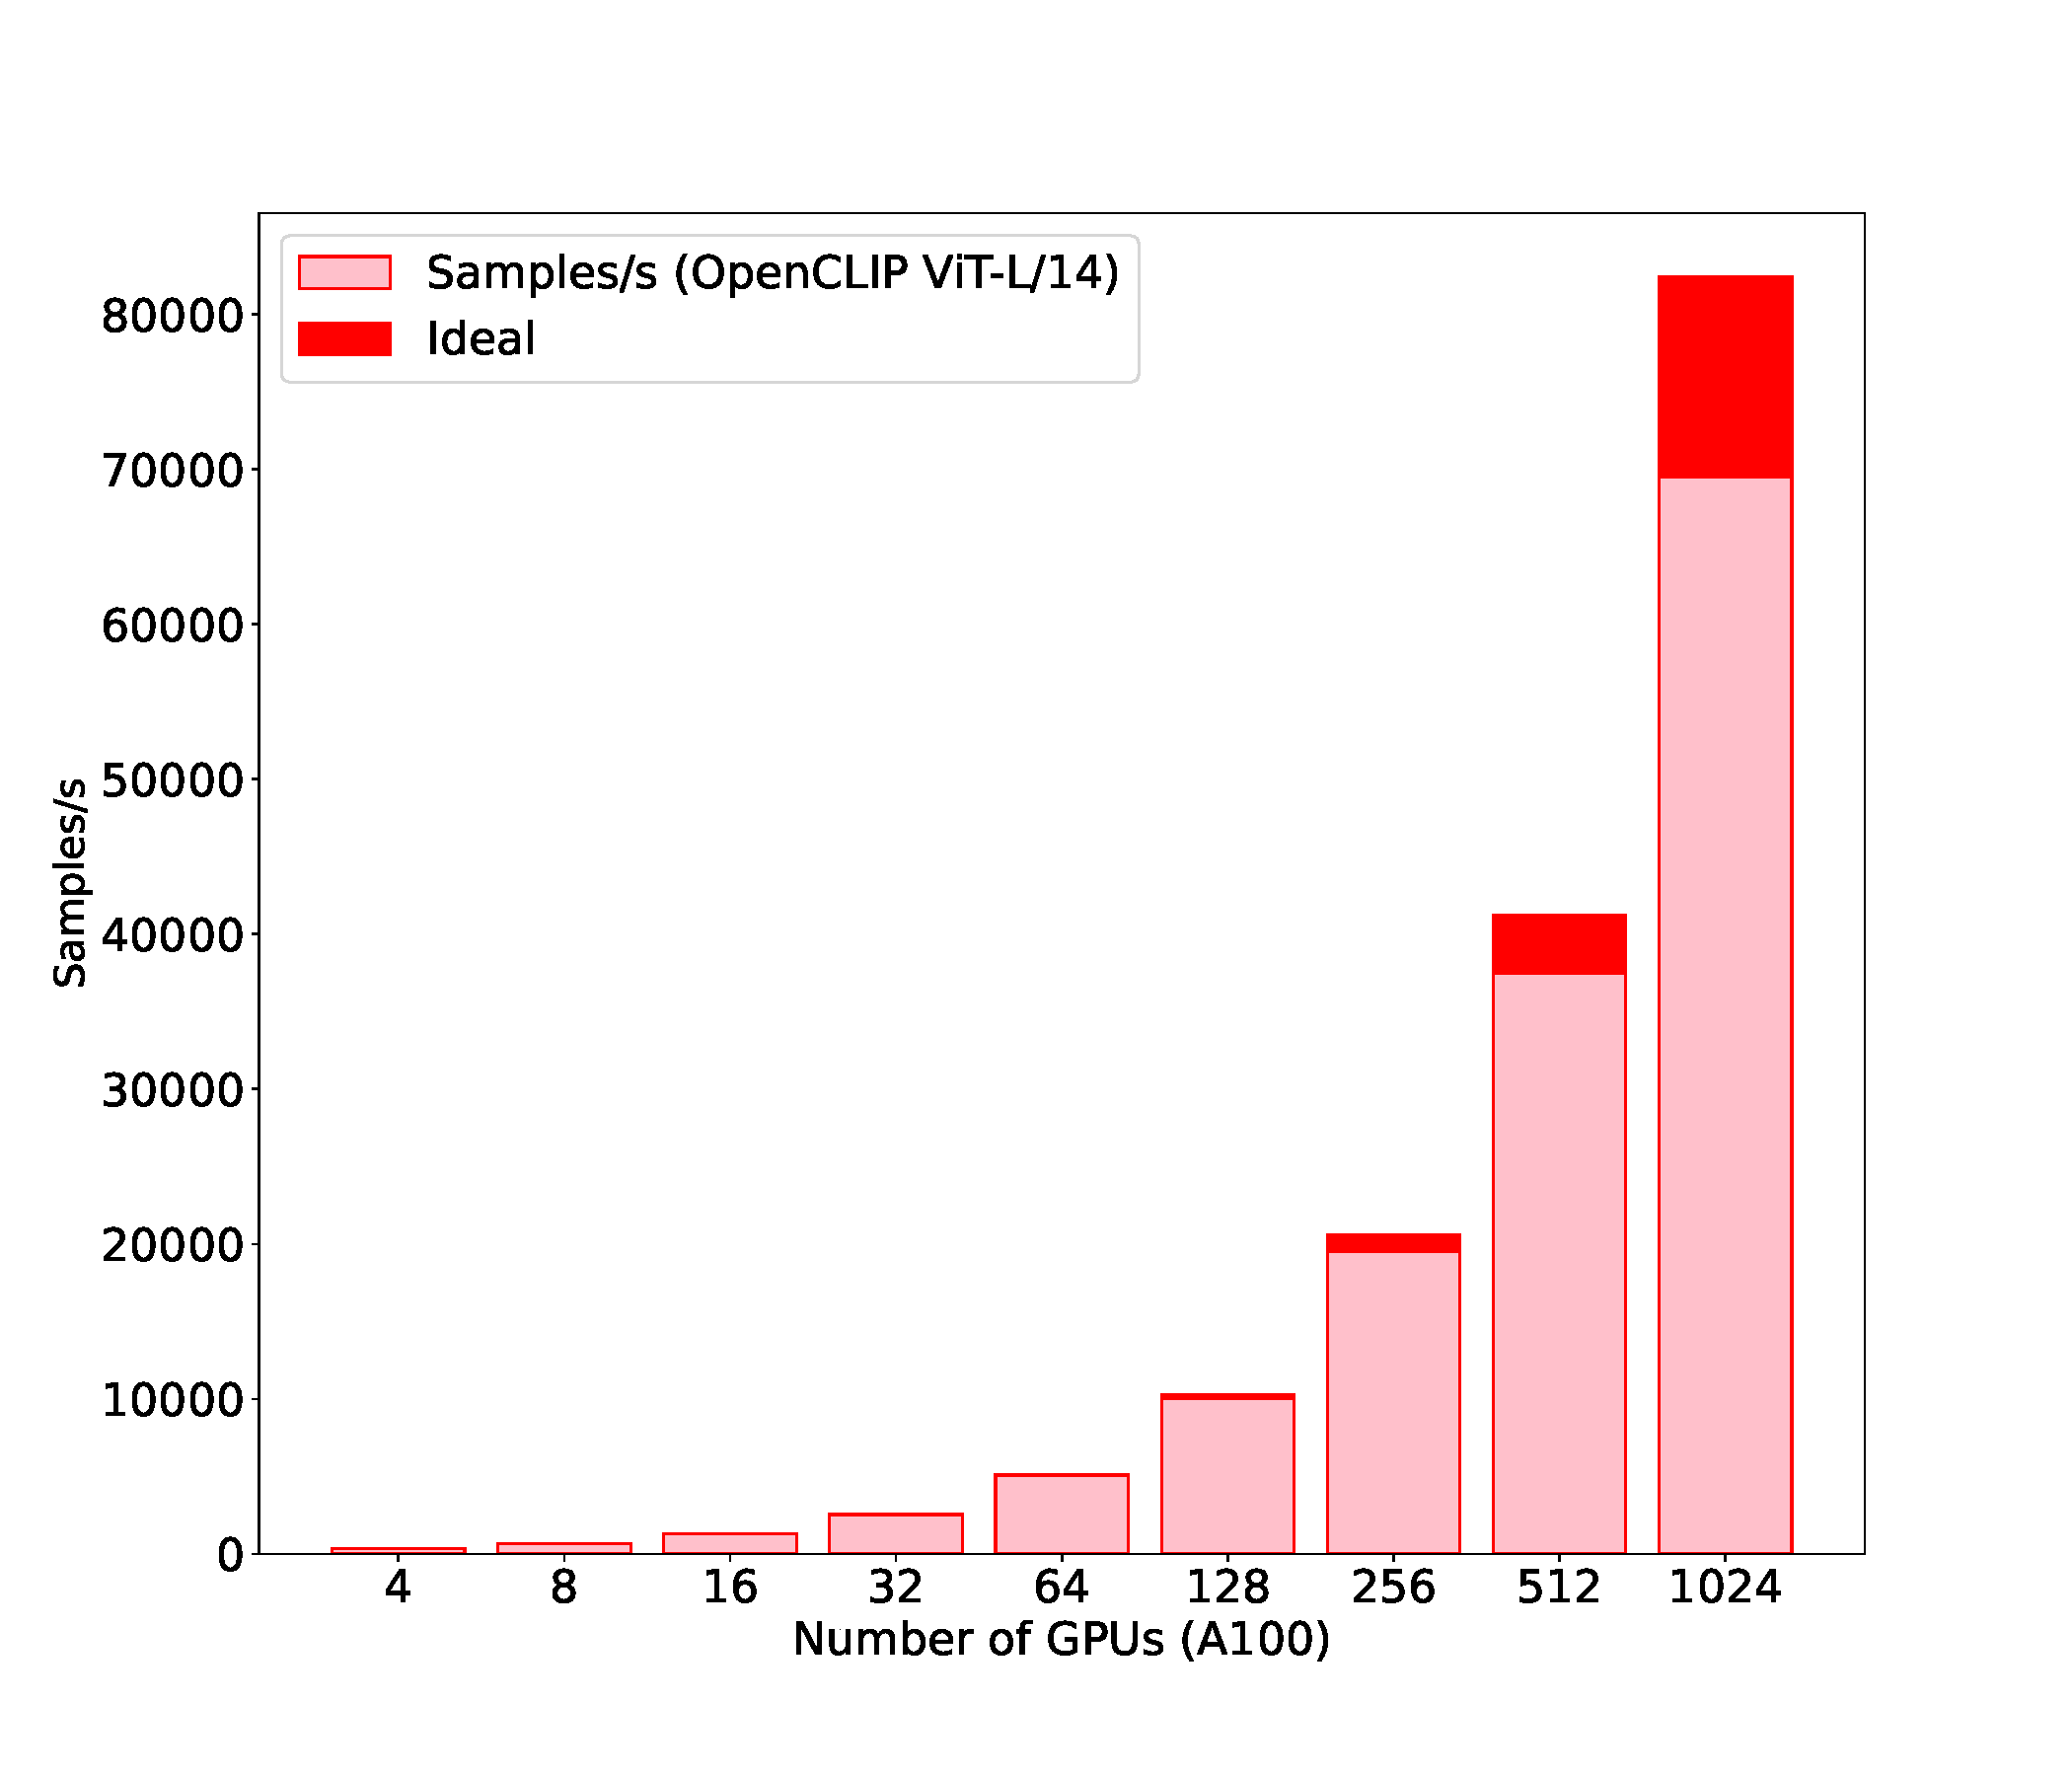
\includegraphics[width=\textwidth]{images/throughput_plot_clip.pdf}
  %\caption{Put your sub-caption here}
  \caption{Throughput in Im/s}
  \label{fig:throughput_clip}
\end{subfigure}
\begin{subfigure}{.5\textwidth}
  \centering
  % include second image
  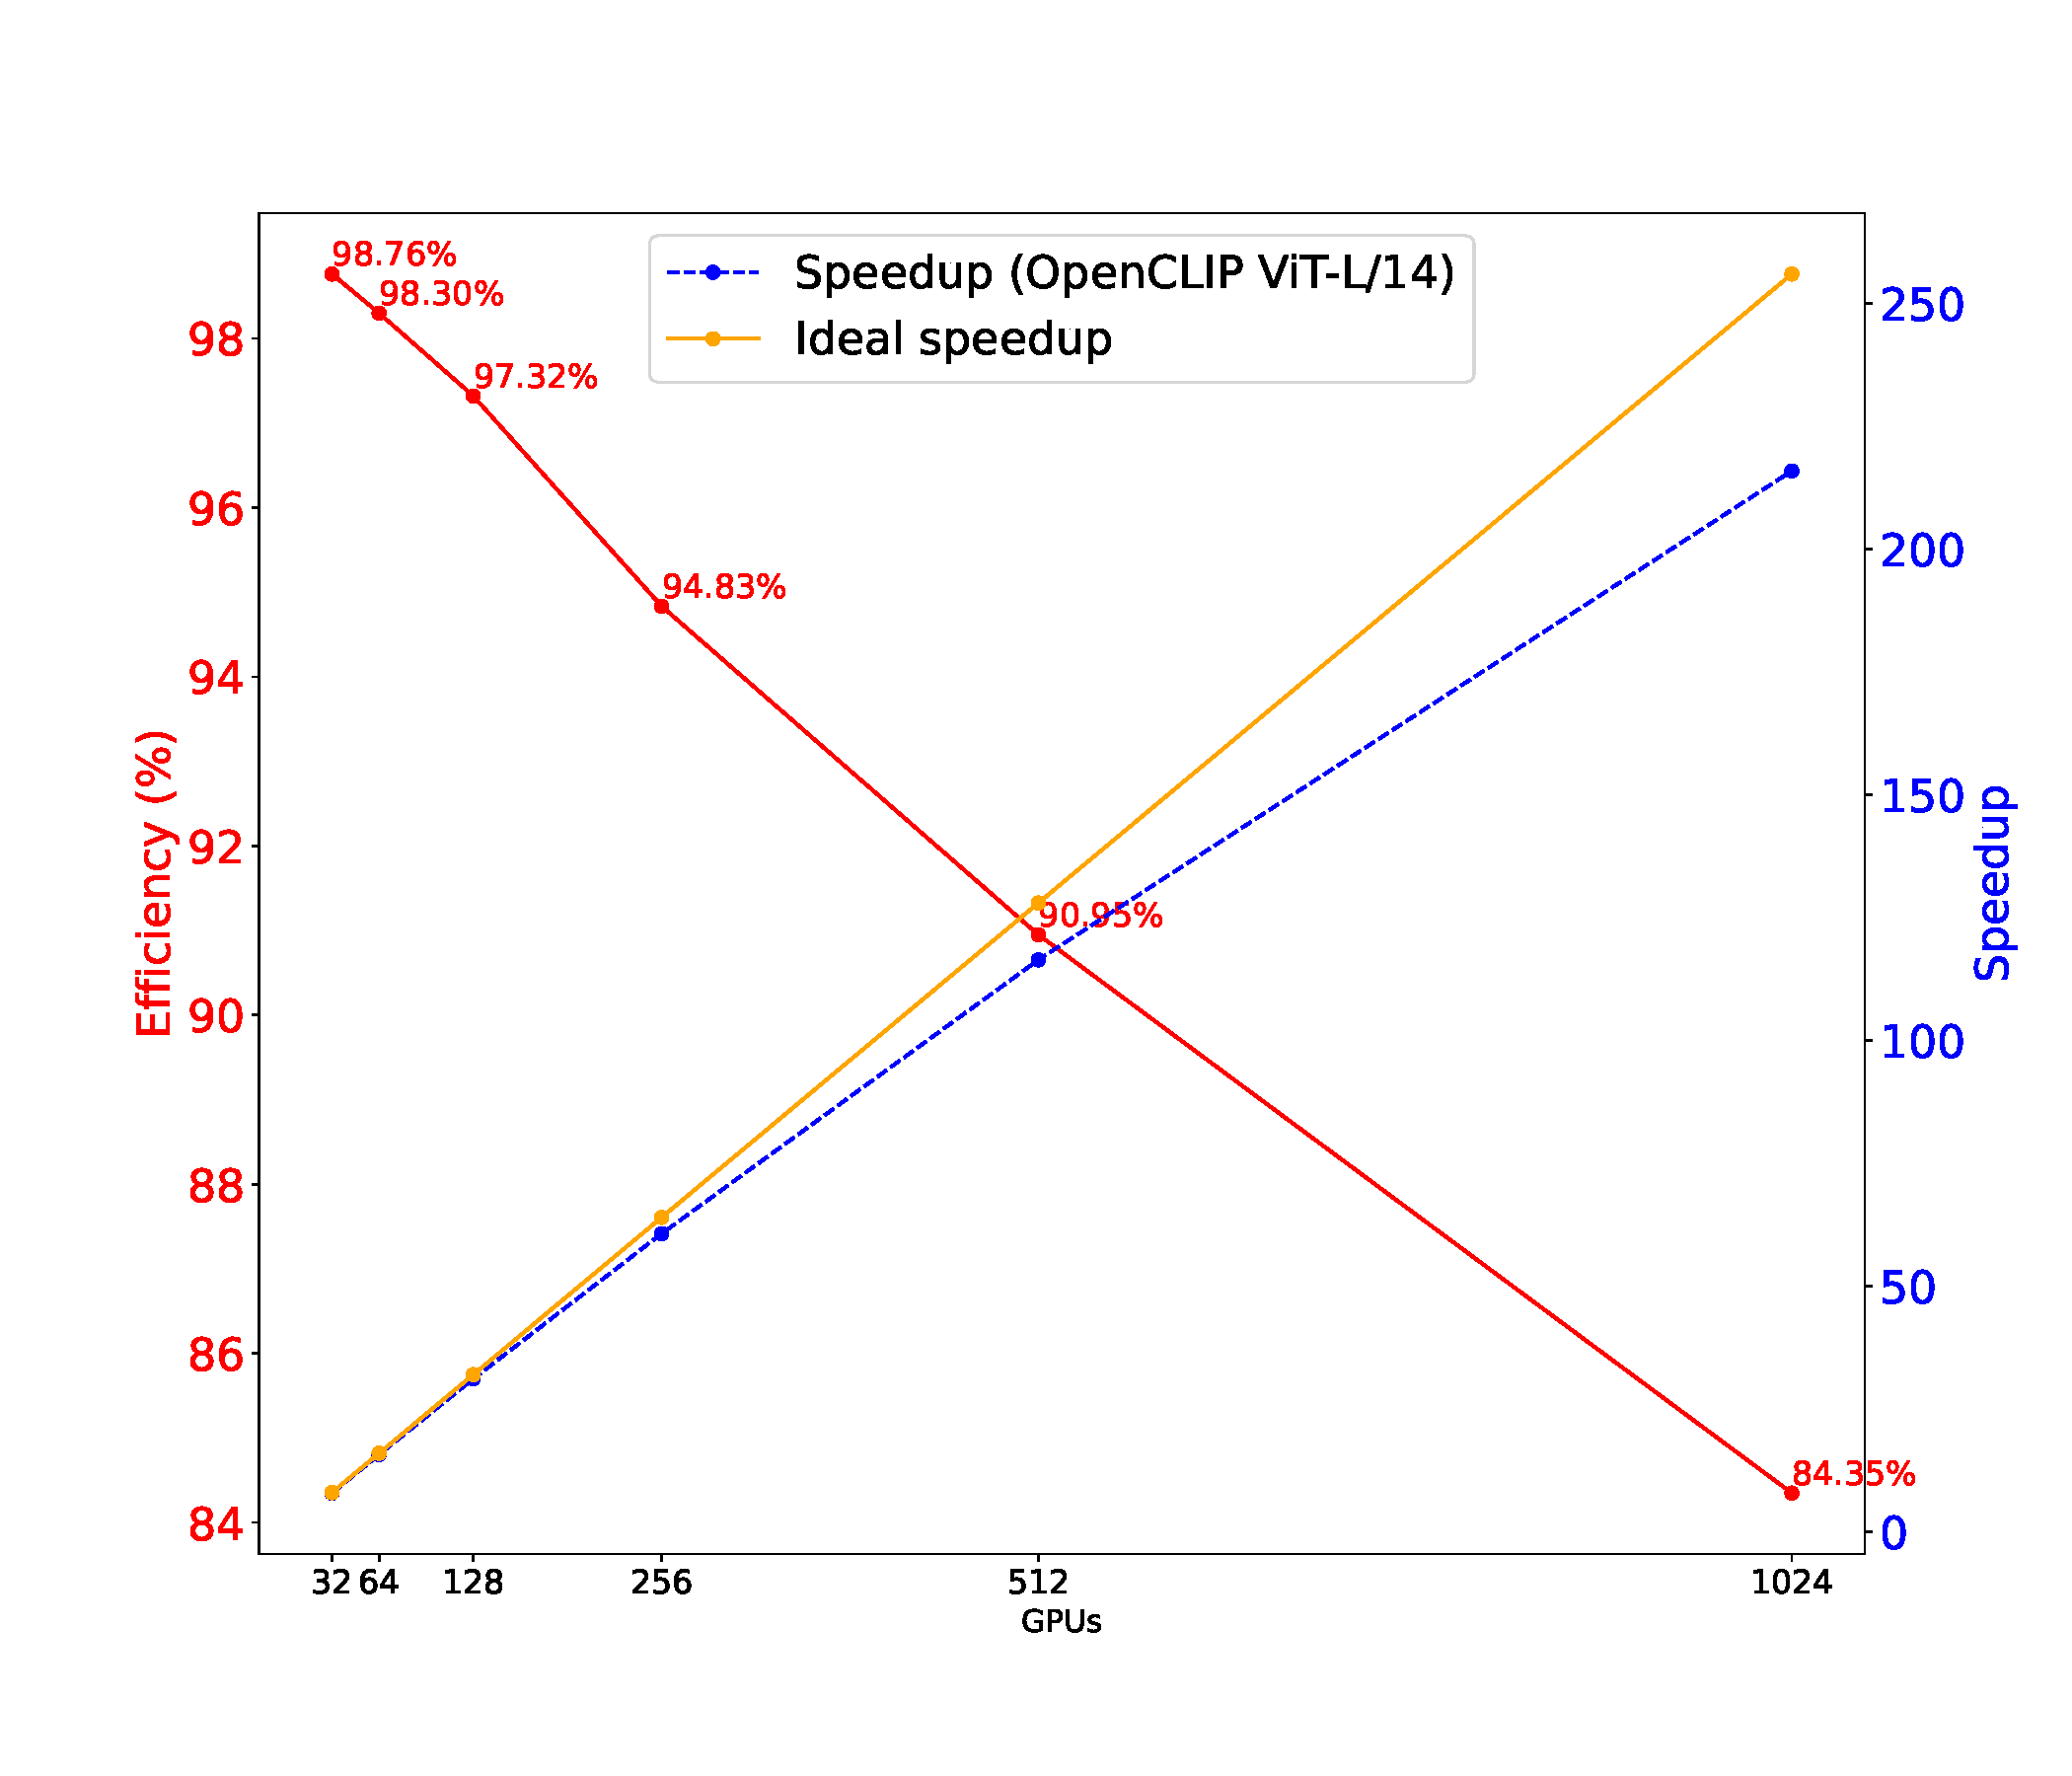
\includegraphics[width=\textwidth]{images/speedup_and_efficiency_plot_clip.pdf}
  %\caption{Put your sub-caption here}
  \caption{Speedup and efficiency}
  \label{fig:speedup_clip}
\end{subfigure}
%\vspace*{-0.2cm}
\caption{Distributed training for OpenCLIP ViT-L/14, scaling behavior on the supercomputer using A100 GPUs while varying the number of GPUs. In Figure~\ref{fig:throughput_clip},  we  show  the  raw throughputs and in Figure~\ref{fig:speedup_clip} we show speedup and efficiency we obtain in the same setup, relative to training with a single node (each node contains 4 GPUs).}
\label{fig:scaling_R152}
\end{figure}

% \caption{Distributed training for OpenCLIP ViT-L/14, scaling behavior on JUWELS Booster using A100 GPUs while varying the number of GPUs. In Figure~\ref{fig:throughput_clip},  we  show  the  raw throughputs and in Figure~\ref{fig:speedup_clip} we show speedup and efficiency we obtain in the same setup, relative to training with a single node (each node contains 4 GPUs).}


% A pre-training with large R152x4 on takes about 81 hours on ImageNet-21k and x hours on ImageNet-1K with $256$ A100 GPUs, while pre-training with small R50x1 

\subsection{Sharding contrastive loss}

The InfoNCE loss \cite{oord2018representation} used by CLIP can be thought of as a method to maximize the mutual information between text and image representations. Formally, Oord et al. express that $I(X;Y)\geq \log(N)-\mathcal{L}_N$, $N$ denoting batch size and $\mathcal{L}_N$ representing the InfoNCE loss. As a result of this lower bound, maximizing the batch size will maximize our mutual information.

Radford et al. \citep{radford2021learning} take advantage of this bound and use $N=32,768$ to train CLIP. Such a batch size necessitates the sharding of computation. Although the original CLIP paper points towards this notion, the implementation details are nontrivial.

Before sharding, the similarity scores will take up $\mathcal{O}(N^2)$ memory on each worker, totalling to 4 GB of VRAM in FP32. After sharding memory reduces to instantiating two $n\times N$ matrices, $n$ being the batch size allocated to each worker. Using a local batch size of 256, the similarity matrices now occupy 64 MB of memory in FP32.

To achieve this memory reduction, we can eliminate redundant computations and compute the similarities of local features versus all features. When aggregated across all machines, this achieves identical gradients. However, it should be noted that the all-gather method is imperative for correct gradient calculation. PyTorch's standard \texttt{torch.distributed.all\_gather} can not be differentiated through, while \texttt{torch.distributed.nn.functional.all\_gather} can be. Thus, we require the use of the latter to correctly calculate the gradients in a distributed manner.


\subsection{Training instabilities}

As parameterization increased within our training runs, so did model model instability. Half-way through the runs of ViT L/14 H/14 and g/14, NaN values and loss spikes began occurring.

To address these issues, we attempted to use extra normalization layers, add scaled cosine attention, resume many steps before crashes, and implement other architecture tweaks with no success. What ended up solving the stability issues was increasing precision.

Using Automatic Mixed Precision (AMP) with bfloat16 over float16, or float32 with tensor-float32 resolved the issues mentioned above. We also have observed that even the smaller ViT-B models with AMP can become unstable when learning rate and batch size become sufficiently large, suggesting a generic scheme behind the phenomenon where frequency of instabilities occurring during the training is a function of model scale and global batch size.

\section{Experimental details}
\label{sec:appendix:experiments}

\subsection{Datasets employed in experiments.}
\label{sec:appendix:datasets}

\textbf{LAION-400M and LAION-5B.} Both LAION-400M \citep{schuhmann2021laion} and LAION-5B \citep{Schuhmann2022} are open, public image-text datasets that were composed by obtaining links from Common Crawl \citep{common_crawl}. While LAION-400M contains 414M english image-text pairs, LAION-5B is currently the largest public image-text dataset containing over 5.8 billion multi-lingual image-text examples. In both cases, samples are obtained by filtering a subset of Common Crawl with a pre-trained OpenAI ViT B/32 model. LAION-5B contains an English image-text subset of 2.32 billion samples, to which we refer as LAION-2B in this work. Besides the open nature of the datasets, a further advantage is full transparency about the dataset composition and assembly, with software stack and tools around LAION-400M and LAION-5B released as open-source, increasing reproducibility of experiments. This already resulted in numerous works using the datasets for training state-of-the-art language-vision models \citep{rombach2021highresolution, mustafa2022multimodal, ho2022imagen, wang2022internimage, fang2022eva}, %which also provides a validation for using those datasets for studying scaling laws in this work.  
validating the usage of those datasets for studying scaling laws in this work.

\begin{table}
\centering
        \begin{footnotesize}
        \rowcolors{2}{light-light-gray}{white}
        \begin{tabular}{cc}\hline
        \textbf{Dataset}  & \textbf{\# English Img-Txt Pairs} \\
        \hline
        \multicolumn{2}{c}{\textbf{Public Datasets}}         \\ \hline
        {LAION-400M} & 407M \\
        {LAION-2B} & 2.3B                    \\ \hline
        \multicolumn{2}{c}{\textbf{Private Datasets}}         \\ \hline
        CLIP WIT (OpenAI) & 400M                    \\
        ALIGN    & 1.8B                    \\
        BASIC    & 6.6B                      \\ \hline
        \end{tabular}
        \end{footnotesize}

  \caption{\textbf{Open LAION datasets used for pre-training in this study.} Adapted from \citep{Schuhmann2022}. LAION-2B is a subset of multi-lingual LAION-5B and is more than 20 times larger than other public English image-text datasets. The scale of LAION-2B is comparable to the largest private dataset used for language-vision model training.}%
  \label{fig:laion_datasets}
\end{table}

\textbf{Downstream transfer and fine-tuning datasets.} For downstream classification tasks, in addition to standard ImageNet, we follow~\cite{Schuhmann2022} and use VTAB+, a collection of datasets in VTAB together with ImageNet derived robustness datasets and additional datasets, forming a comprehensive set of 35 tasks. For evaluating retrieval, we make use of MS-COCO and Flickr30K. For fine-tuning, we make use of a dedicated ImageNet-12k dataset  (12M training examples, 470K validation examples) which is a subset of the full ImageNet-22k (14M examples) that we employ for the multi-stage fine tuning procedure described in Sec. \ref{subsect:scaling_laws_finetune}. For more details on downstream datasets, refer to Table \ref{tab:datasets_list}.

%ToDo Mehdi (DONE)
\textbf{Duplication check for pre-training and downstream datasets.}. To ensure that images from downstream datasets are not contained in LAION, we conduct a simple
duplication check based on the perceptual image hash library pHash~\cite{zauner2010implementation}.
We apply pHash's discrete cosine transform (DCT) method on LAION-400M images and images from downstream datasets. Afterwards, for each downstream dataset, we count the number of duplicates by finding the hashes that are also present in LAION-400M. We provide the overlap percentage found on a subset of  downstream datasets in Table~\ref{table:dups}. In Figure~\ref{fig:dups_viz}, we also provide a sample of images from downstream datasets detected as duplicates in LAION-400M. Overall, the ratio of detected duplicates is around 1\%, except on ImageNet-R (3.80\%) and ImageNet-Sketch (5.15\%). We investigate further and re-evaluate zero-shot performance of our pre-trained Vit-H/14 on ImageNet-R and ImageNet-Sketch by removing duplicates from their test sets. For ImageNet-R, zero-shot top-1 accuracy goes from 89.32\% to 89.21\% after removing duplicates. For ImageNet-Sketch, zero-shot top-1 accuracy goes from 66.57\% to 66.59\% after removing duplicates.
%This amount of duplicates is still low, and the two datasets do not have significant impact on scaling laws trends observed here. 
We conclude, based on those results, that it is unlikely that downstream results would be affected by the duplicates. This would be in line with previous works\citep{radford2021learning, zhai2021lit} which explicitly measured and compared performance on deduplicated downstream datasets, reporting that duplication in test sets do not significantly alter most results. This is likely due to the very large scale and diversity of pre-training data. We leave more elaborated duplication detection procedures for future work. 

% We investigate further those two datasets and find XXX.

\begin{table}
\centering
\rowcolors{2}{light-light-gray}{white}
\begin{tabular}{ll}
\toprule
           \textbf{Dataset} &    \textbf{Overlap\%} \\
\midrule
       ImageNet & 1.02 \\
    ImageNet-v2 & 1.35 \\
     ImageNet-R & 3.80 \\
ImageNet Sketch & 5.15 \\
     ImageNet-A & 0.40 \\
      ObjectNet & 0.10 \\
      CIFAR-100 & 0.02 \\
       CIFAR-10 & 0.03 \\
        MS-COCO & 1.12 \\
      Flickr30K & 1.30 \\
\bottomrule
\end{tabular}
\caption{Ratio of images (\%) on downstream datasets that were detected on LAION-400M, using pHash~\cite{zauner2010implementation}.}
  \label{table:dups}
\end{table}


\begin{figure}[ht]
\centering
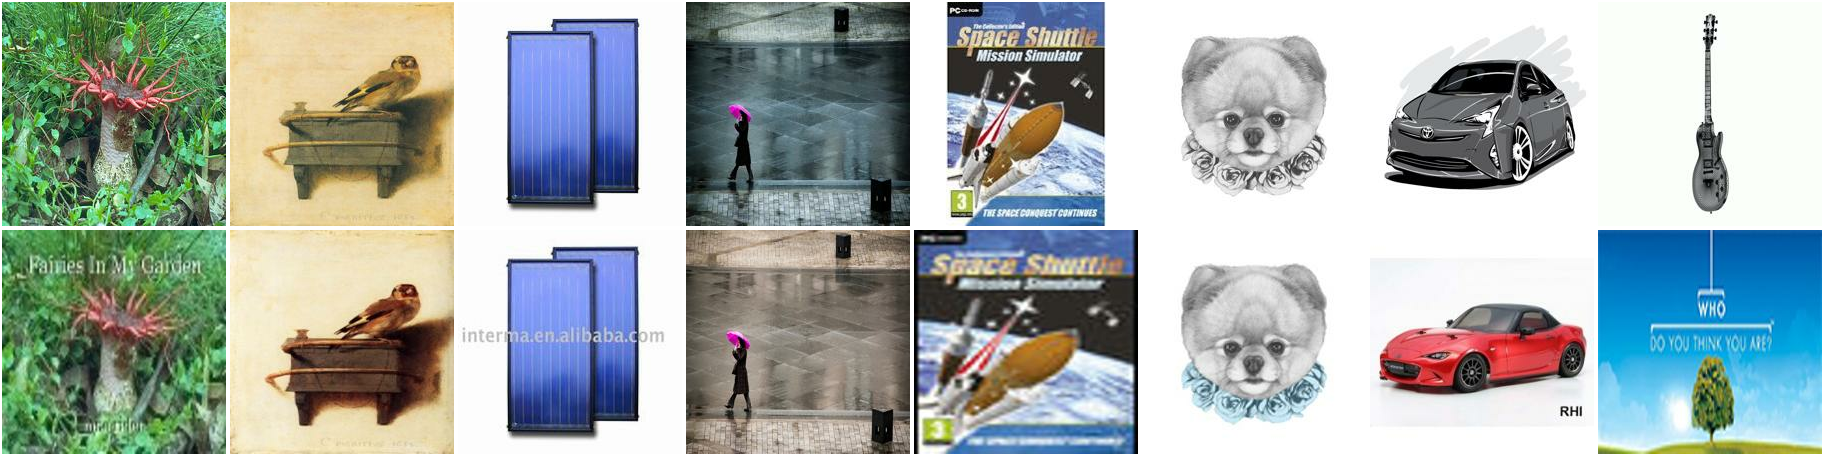
\includegraphics[width=\textwidth]{images/dups_grid.png}
%\caption{Put your sub-caption here}
\caption{Duplicate images detected using pHash\cite{zauner2010implementation} between downstream datasets and LAION-400M. Top row shows images from downstream datasets, while bottom row show corresponding detected duplicates in LAION-400M. We observe near-duplicate detection for a variety of image transformations: blurring, text blitting, color transformations, cropping, and scaling.
Last two columns show false positive examples detected on ImageNet-Sketch dataset. In general, we observed that most of false positive cases had a uniform background, which pHash seems to be sensitive to.
}
\label{fig:dups_viz}
\end{figure}


% LAION-400M was already successfully used by various works on language-vision modelling, further underpinning its suitability for systematic scaling law studies. 

% LAION-400M\citep{schuhmann2021laion} and LAION-5B\citep{Schuhmann2022} are open, public image-text datasets validated by pre-training of state-of-the art multi-modal models like CLIP\citep{radford2021learning} and Stable Diffusion\citep{rombach2021highresolution}. LAION-5B contains an English image-text subset of 2.32 billion samples, to which we refer as LAION-2B in this work.  Due to its transparency and open-source nature of software stack and tools released for dataset reproduction, LAION-400M was already successfully used by various works on language-vision modelling, further underpinning its suitability for systematic scaling law studies. 


% Besides the open nature of the datasets, a further advantage is full transparency about the dataset composition and assembly, with software stack and tools released as open-source, increasing reproducibility of experiments.
% around LAION-400M and LAION-5B 

% LAION-400M\citep{schuhmann2021laion} and LAION-5B\citep{Schuhmann2022} are open, public image-text datasets validated by pre-training of state-of-the art multi-modal models like CLIP\citep{radford2021learning} and Stable Diffusion\citep{rombach2021highresolution}. Both datasets were composed by obtaining links from Common Crawl\citep{common_crawl}. While LAION-400M contains 414M image-text pairs, LAION-5B is currently the largest public image-text dataset containing over 5.8 billion examples. In both cases, samples are obtained by filtering a subset of Common Crawl with a pre-trained OpenAI ViT B/32 model. LAION-5B contains an English image-text subset of 2.32 billion samples, to which we refer as LAION-2B in this work. Besides the open nature of the datasets, a further advantage is full transparency about the dataset composition and assembly, with software stack and tools around LAION-400M and LAION-5B released as open-source, increasing reproducibility of experiments. LAION-400M was already successfully used by various works on language-vision modelling, further underpinning its suitability for systematic scaling law studies. 

% \footnote{\url{http://commoncrawl.org/}}
% Moreover, their CLIP embeddings, and kNN indices that allow efficient similarity search ...
% \textbf{Large-scale multi-modal LAION-400m dataset.} Multi-modal language-vision models like CLIP are trained on hundreds of millions of image-text pairs and then show remarkable capability to perform zero- or few-shot learning and transfer even in the absence of per-sample labels on target image data.
%Despite this trend, until the release of our LAION-400M dataset~\cite{Schuhmann2021} there had been no publicly available dataset of sufficient scale for training such models from scratch and studying their transfer capabilities, also with regard to the effect of training scale.
%To address this issue, we built and released the public LAION-400M dataset, containing 414 million CLIP-filtered image-text pairs, their CLIP embeddings, and kNN indices that allow efficient similarity search. This large-scale dataset will be a cornerstone for studying the effect of data scale on downstream transfer performance in this project. 


% Specifically, we introduce LAION-5B, the largest public image-text dataset containing over 5.8 billion examples (see Table \ref{fig:sub2} for a comparison).
% By starting from Common Crawl \citep{common_crawl} and filtering this data source with an existing CLIP model, we derive a dataset consisting of three parts: 2.32 billion English image-text examples, 2.26 billion multilingual examples, and 1.27 billion examples that are not specific to a particular language (e.g., places, products, etc.).
%Beyond assembling the dataset, we also explore its ethical implications and flaws that emerge with large-scale data collection.
%By releasing LAION-5B publicly, we offer the first opportunity for the community to audit and refine a dataset of this magnitude. 

%To validate that LAION-5B is indeed suitable for training large image-text models, we conduct multiple experiments.
%We focus on matching the performance of OpenAI's CLIP models because they are the largest publicly released image-text models.
%OpenAI's CLIP models were trained on 400~million image-text pairs, and hence we also train CLIP models on a subset of LAION-5B containing the same number of examples (``LAION-400M'').
%Across a diverse range of problem settings including ImageNet (zero-shot), distribution shifts, VTAB, retrieval, and fine-tuning, our models trained on LAION-400M match or come close to the performance of OpenAI's CLIP models.
%Our ViT-L/14 models trained with OpenCLIP are the first open source reproductions of the largest CLIP models released by OpenAI.

% Hence we do not only release our dataset, but also our software stack we built for assembling LAION-5B.
% We view our initial data release and this paper as a first step on the way towards a widely applicable pre-training dataset for multimodal models.


\subsection{Further experimental results}
\label{sec:appendix:exp_further_results}

\subsubsection{Predictions derived from scaling laws}
\label{sec:appendix:predictions}
%TODO: here predictive scaling plots, at least for zero-shot imagenet-1K and retrieval (DONE)

\begin{figure}[ht]
\begin{subfigure}{.5\textwidth}
  \centering
  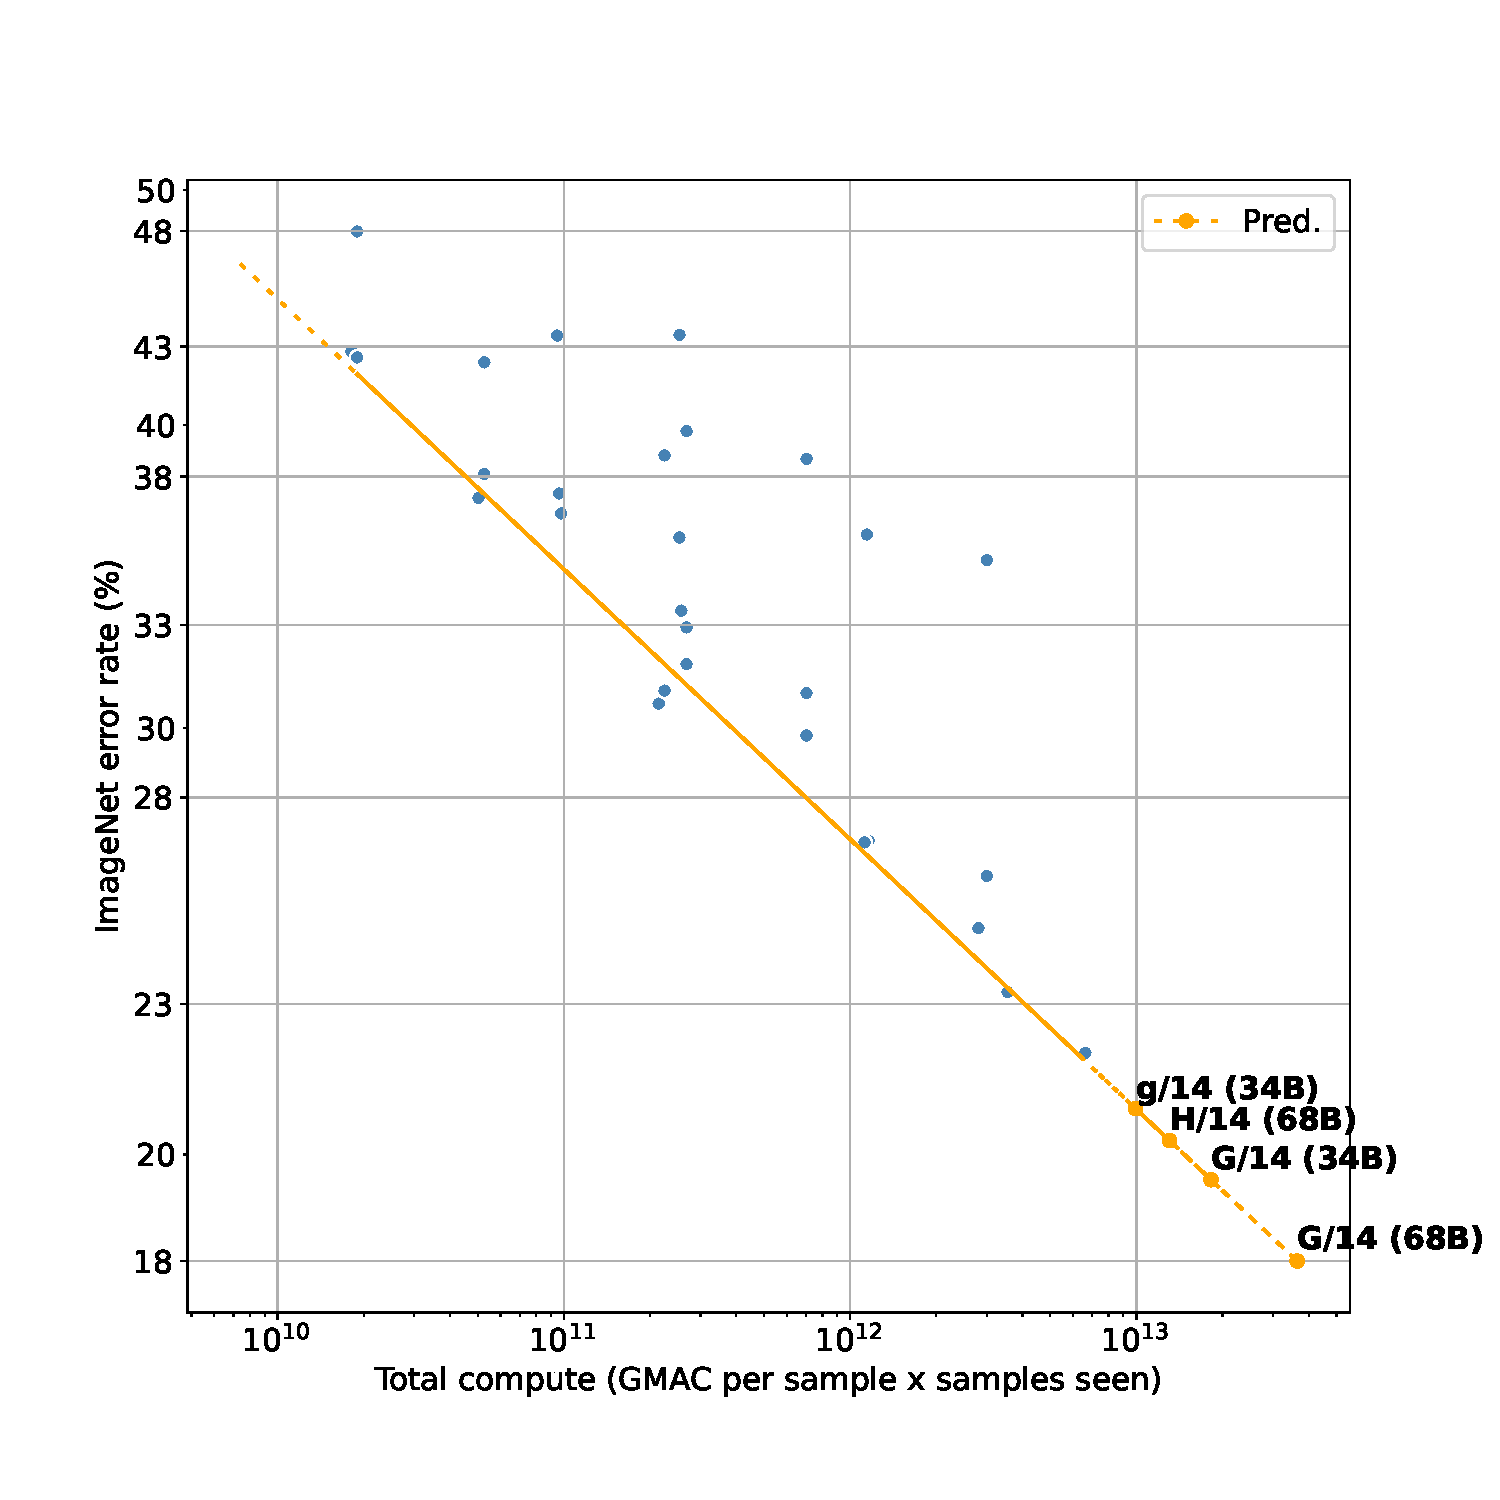
\includegraphics[width=\textwidth]{images/prediction_plot_imagenet1k.pdf}
  %\caption{Put your sub-caption here}
  \caption{Predictions on ImageNet}
  \label{fig:predictionplot_imagenet}
\end{subfigure}
\begin{subfigure}{.5\textwidth}
  \centering
  % include second image
  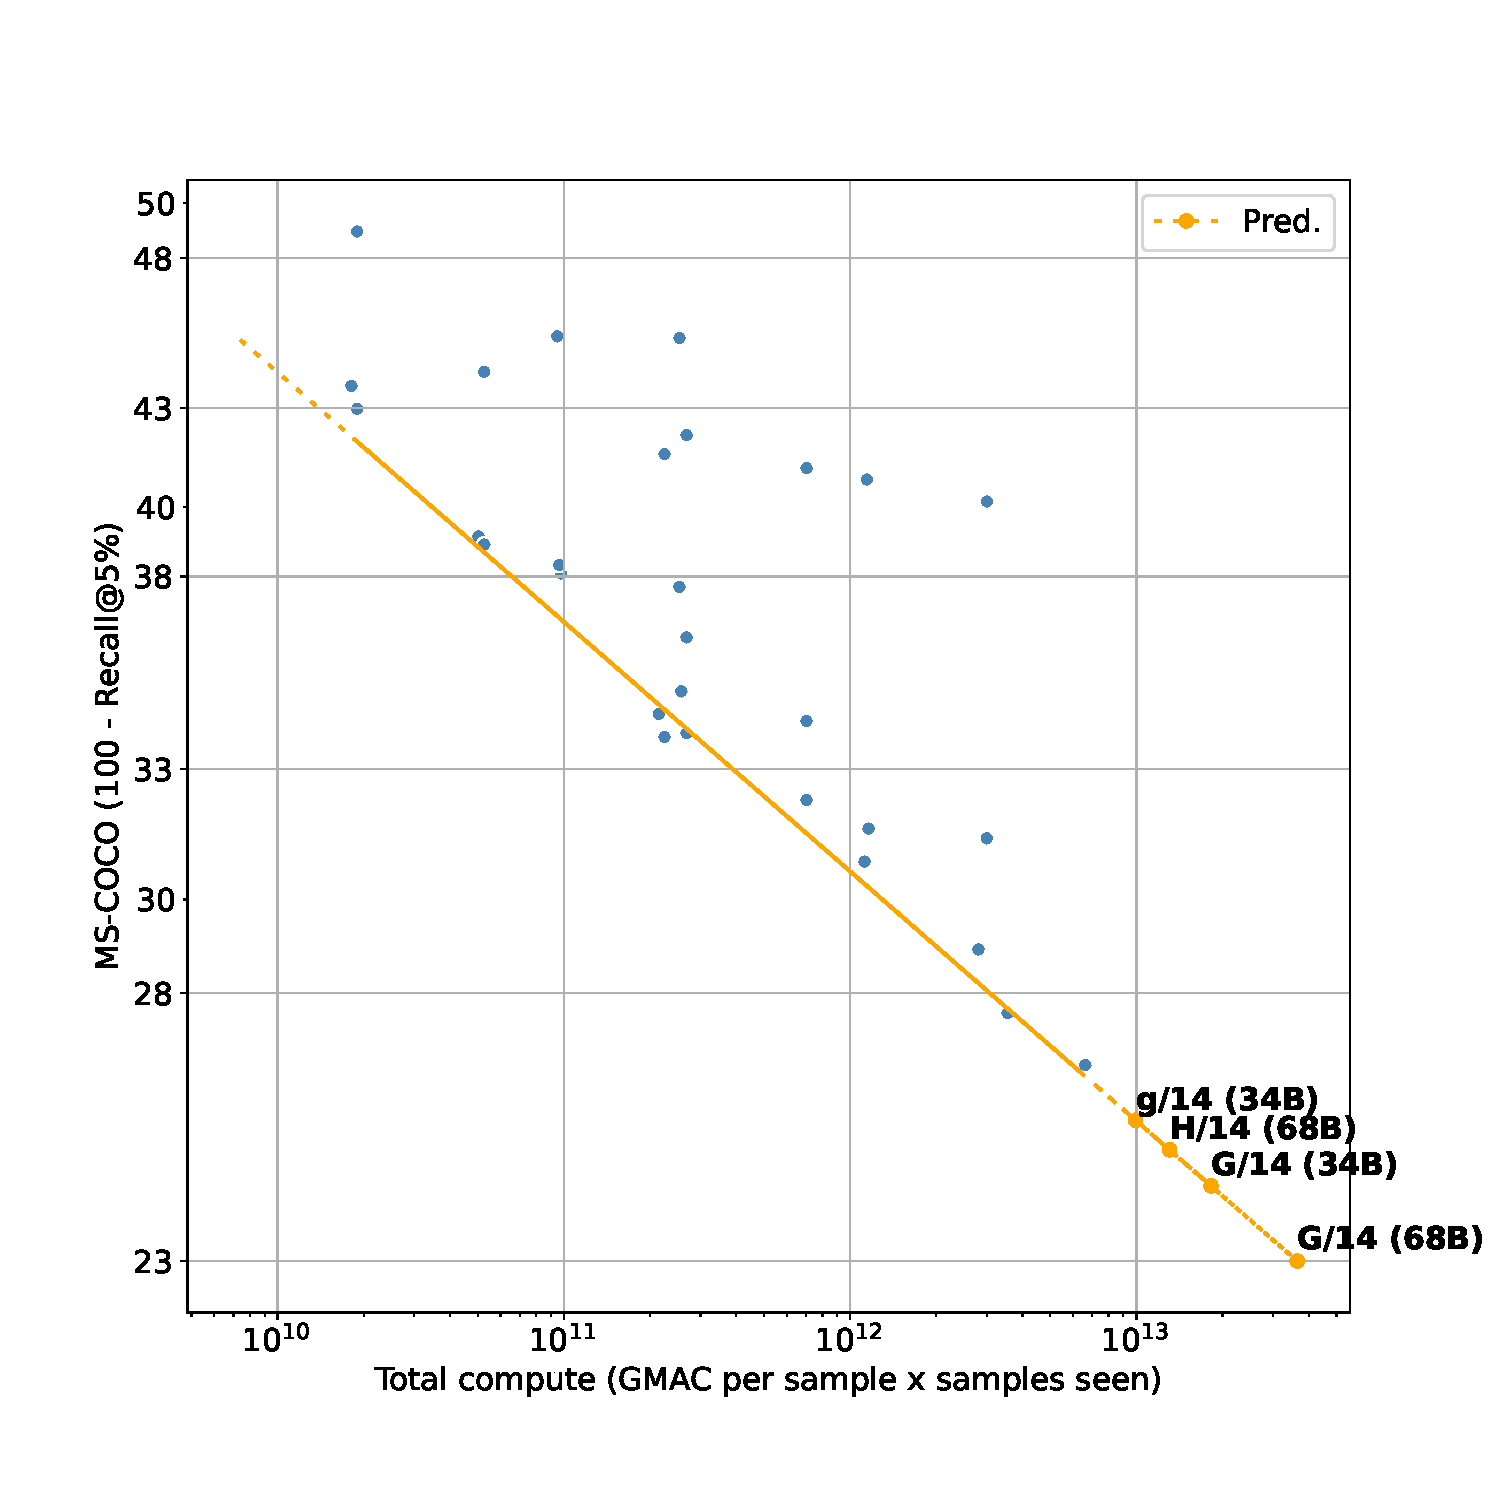
\includegraphics[width=\textwidth]{images/prediction_plot_mscoco_captions.pdf}
  %\caption{Put your sub-caption here}
  \caption{Predictions on MS-COCO}
  \label{fig:predictionplot_coco}
\end{subfigure}
%\vspace*{-0.2cm}
\caption{Zero-shot performance extrapolation of g/14, H/14 and G/14 on larger scales. We fit a power-law on the Pareto frontier of available models. In Fig.\ref{fig:predictionplot_imagenet} we show the predictions for ImageNet classification, while in Fig.\ref{fig:predictionplot_coco} we show the predictions for MS-COCO image retrieval.}
\label{fig:predictionplot}
\end{figure}

\begin{table}
%\footnotesize
\centering
\rowcolors{2}{light-light-gray}{white}
\begin{tabular}{cll}
\toprule
\textbf{Model} & \textbf{ImageNet top-1 (\%)} & \textbf{MS-COCO Recall@5 (\%)} \\
\midrule
%H/14 (68B) &              79.73 &             75.03 \\
%g/14 (34B) &              79.11 &             74.48 \\
%g/14 (68B) &              80.66 &             75.85 \\
%G/14 (13B) &              78.26 &             73.75 \\
%G/14 (34B) &              80.47 &             75.68 \\
%G/14 (68B) &              81.92 &             76.99 \\
 H/14 (3B) &       70.78 &            67.58 \\
 g/14 (3B) &       72.11 &            68.65 \\
 G/14 (3B) &       73.93 &            70.12 \\
H/14 (13B) &       75.62 &            71.52 \\
g/14 (13B) &       76.66\textbf{*} &            72.40\textbf{*} \\
G/14 (13B) &       78.26 &            73.75 \\
H/14 (34B) &       77.97\textbf{*} &            73.43\textbf{*} \\
g/14 (34B) &       79.11 &            74.48 \\
G/14 (34B) &       80.47 &            75.68 \\
H/14 (68B) &       79.73 &            75.03 \\
g/14 (68B) &       80.66 &            75.85 \\
G/14 (68B) &       81.92 &            76.99 \\

\bottomrule
\end{tabular}
\caption{Performance extrapolation of g/14, H/14 and G/14 on larger scales corresponding to Fig.\ref{fig:predictionplot}. We fit a
power-law on the Pareto frontier of available models. We show the zero-shot top-1 accuracy predictions for ImageNet and zero-shot retrieval image retrieval Recall@5 predictions for MS-COCO. We denote by  (*) actual measured model performance values, while the rest are predictions.}
\label{table:predictions}
\end{table}



We can use scaling laws derived from our measurements to predict model performance for larger scales on different downstream tasks. To perform predictions, we fit a power-law on the Pareto frontier\footnote{Since total compute budget (measured in GMAC) of different trained models are not exactly aligned, we adopt a binning approach. We bin the GMAC compute budget axis and compute the optimal performance within each bin, then fit a line in log-log space on the resulting bins.}.  Fig.\ref{fig:predictionplot_imagenet} and Fig.\ref{fig:predictionplot_coco} show extrapolation of performance for ImageNet and MS-COCO, respectively. According to the predictions, H/14 (68B samples seen) would achieve 79.73\% (+1.76\%) zero-shot top-1 accuracy on ImageNet and 75.10\% (+1.60\%) image retrieval Recall@5 on MS-COCO, compared to our trained H/14 (34B samples seen).  See also Tab.\ref{table:predictions} for more detailed extrapolation numbers.
For g/14 (68B samples seen), we predict 80.66\% (+4\%) zero-shot top-1 accuracy on ImageNet and 75.85\% (+3.45\%) image retrieval Recall@5 on MS-COCO, compared to our trained g/14 (13B samples seen). 
On the largest compute budget we consider, G/14 (68B samples seen), we predict 81.92\%  zero-shot top-1 accuracy on ImageNet and 76.99\% image retrieval Recall@5 on MS-COCO.
%One way is to predict model performance for a certain model, data and sample seen scale combination. Another way is the predict optimal model performance for a given total compute scale that may correspond to different combinations of model and samples seen scale, across different data scales.

% (Yet Another way is the predict optimal model performance for a given scale (eg model scale) while assuming that other scales (eg data scale and samples seen) can be freely varied )


\subsubsection{Fine-tuning}
\label{sec:appendix:finetuning}

In Table~\ref{table:finetune_results}, we show detailed results of fine-tuning on ImageNet with and without extra data (Imagenet-12k), and show results of the fine-tuned models on five ImageNet robustness test sets.
Also, complementing the results shown in Figure \ref{fig:ft-eight} in Section \ref{subsect:scaling_laws_finetune}, we show a per-task breakdown of the the zero-shot and fine-tuned performance on the eight classification tasks in Figures \ref{fig:ft-eight-zs} and  \ref{fig:ft-eight-ft}. Exact numbers are shown in Tables \ref{tab:appendix:joint_ft_zs}, \ref{tab:appendix:joint_ft_ft}, and \ref{tab:appendix:joint_ft_patch}.


\begin{figure}
    \centering
    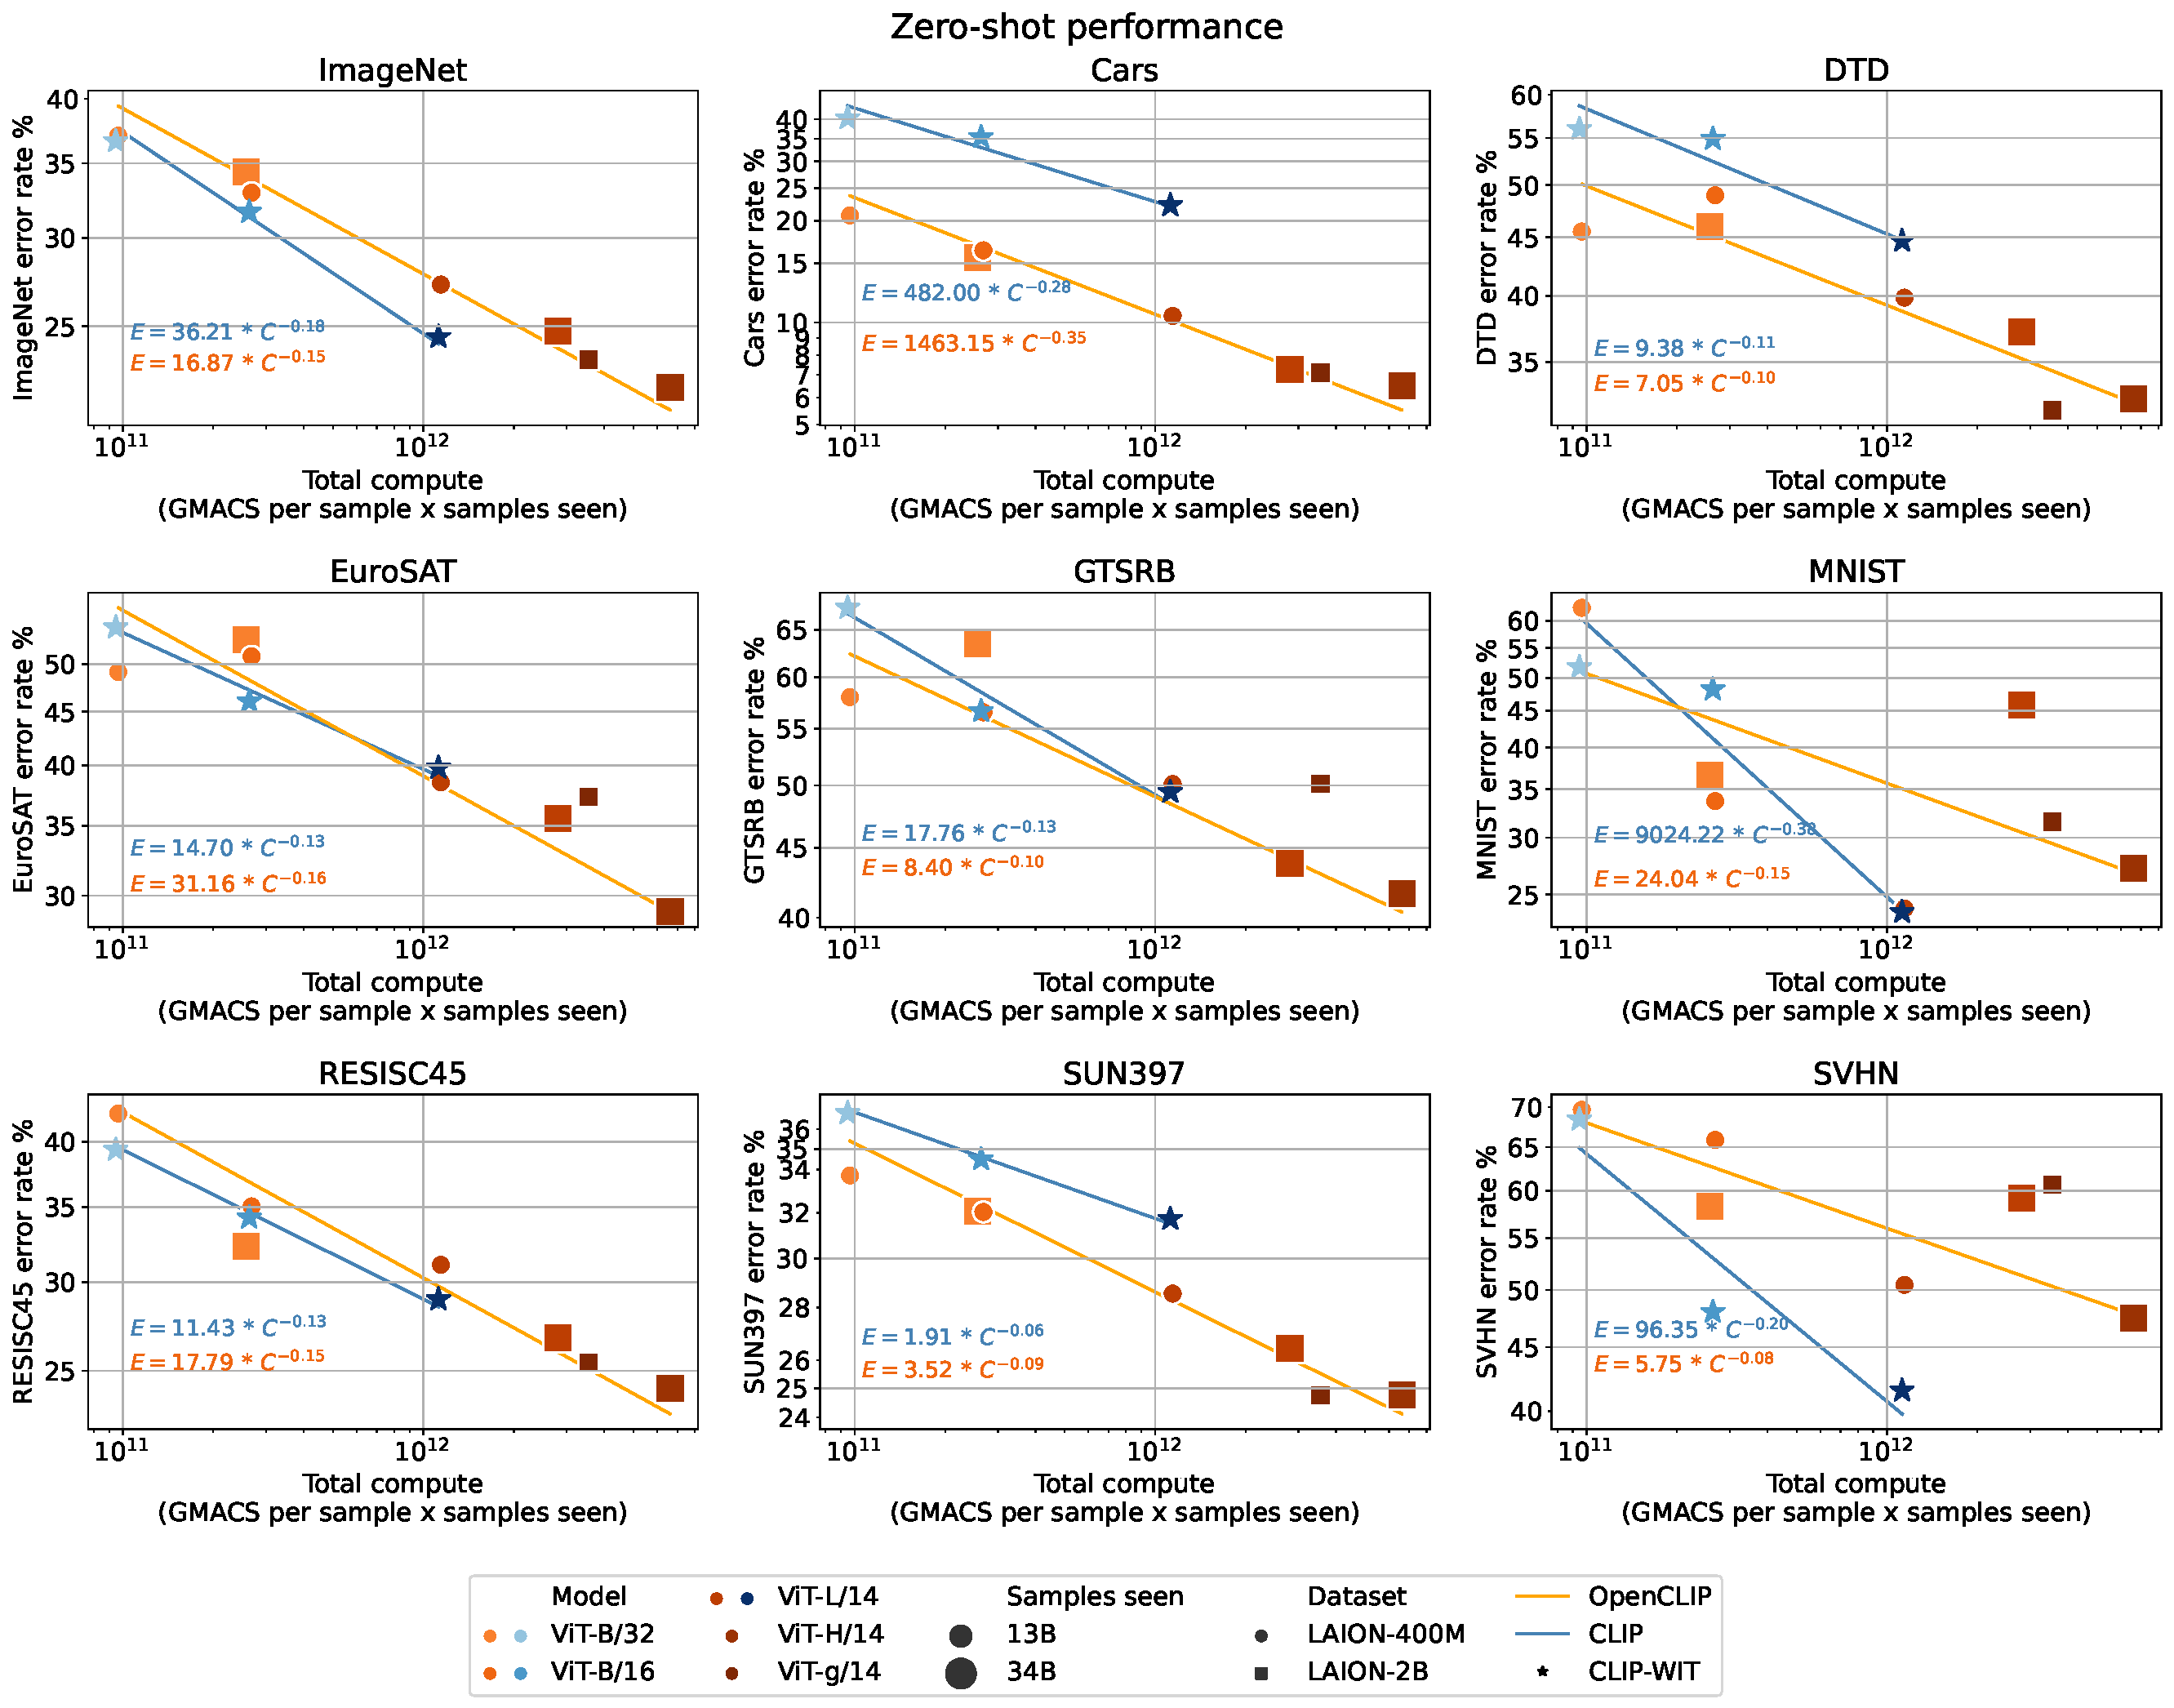
\includegraphics[width=\textwidth]{images/scaling_breakdown_zs.pdf}
    \caption{Scaling trends of zero-shot models on the eight other downstream tasks used for the fine-tuning experiments in Section \ref{subsect:scaling_laws_finetune} and on ImageNet.}
    \label{fig:ft-eight-zs}
\end{figure}
\begin{figure}
    \centering
    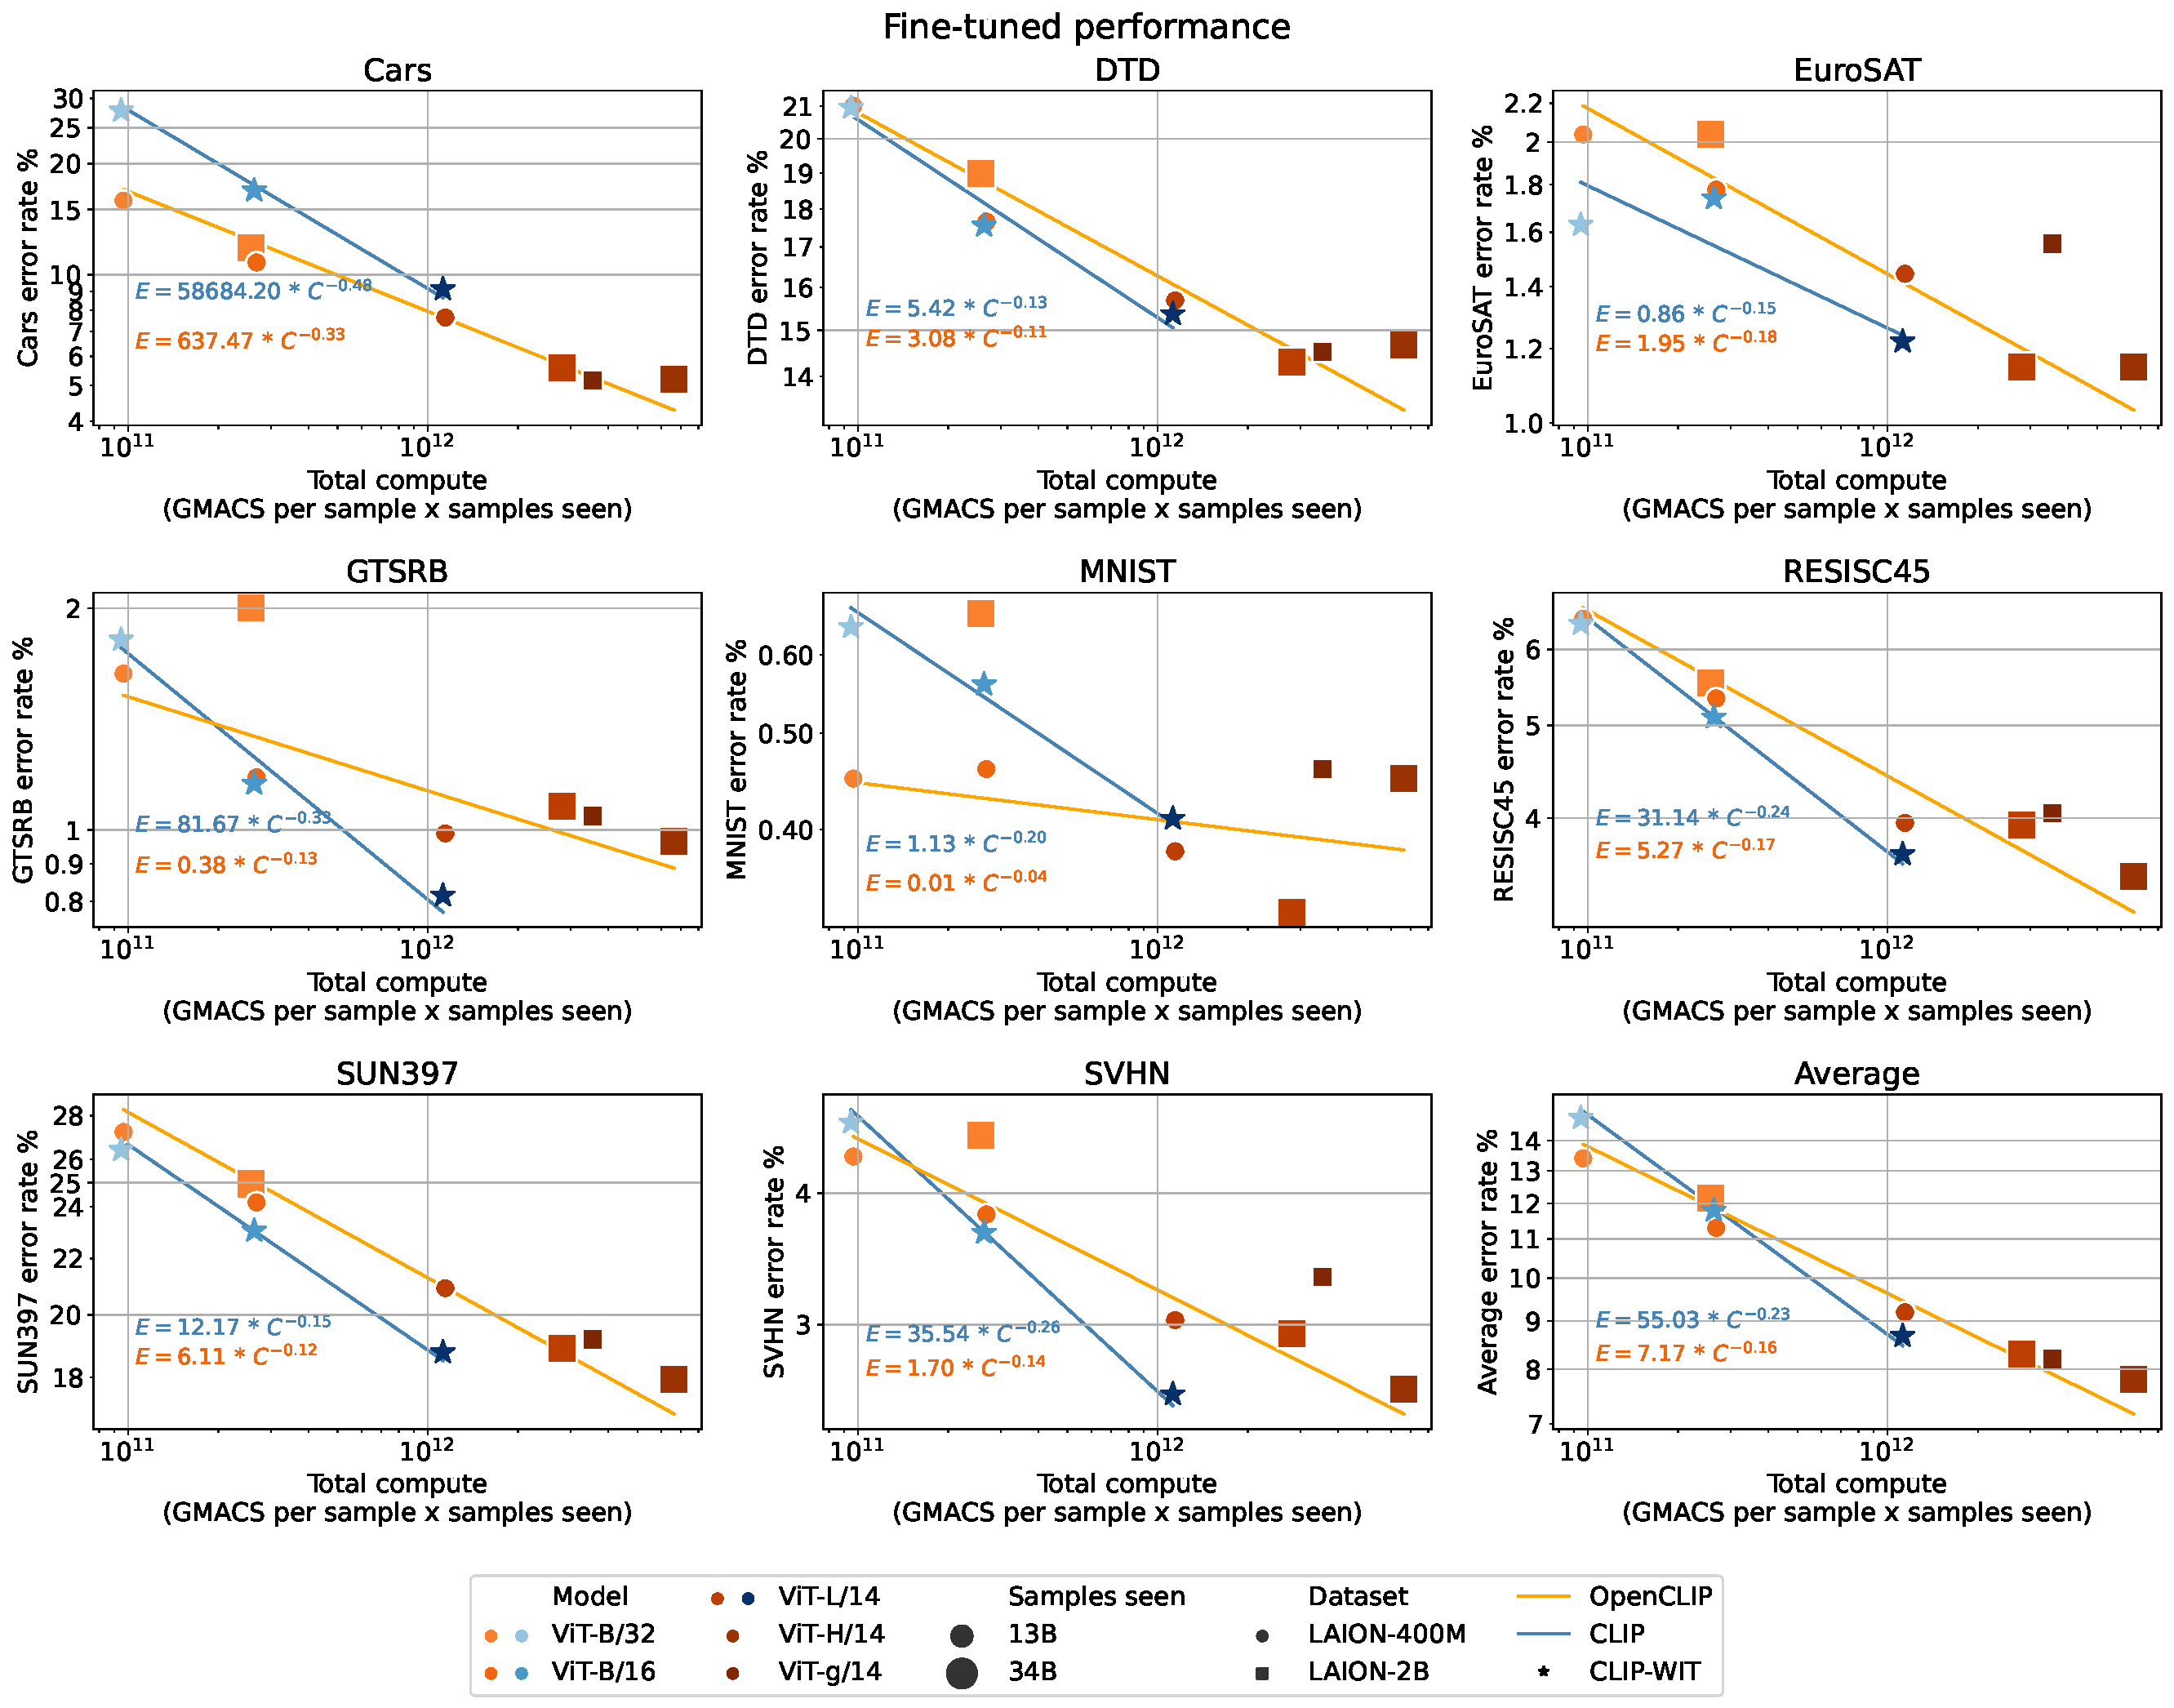
\includegraphics[width=\linewidth]{images/scaling_breakdown_ft.pdf}
    \caption{Scaling trends of fine-tuned models on the eight other downstream tasks used for the fine-tuning experiments in Section \ref{subsect:scaling_laws_finetune}.}
    \label{fig:ft-eight-ft}
\end{figure}



Moreover, since fine-tuning on some downstream tasks can decrease accuracy on others, we experiment with model patching by interpolating between the weights of fine-tuned and zero-shot models, as in Ilharco et al. \cite{ilharco2022patching}.\footnote{The weights $\theta_\textrm{patched}$ of the patched model are obtained via the equation $\theta_\textrm{patched} = (1-\alpha)\theta_\textrm{zero-shot} + \alpha \theta_\textrm{fine-tuned}$, where $\alpha\in[0,1]$ is the mixing coefficient.}
We choose the mixing coefficient $\alpha \in {0, 0.1, ..., 1.0}$ that maximizes average accuracy on the eight downstream tasks, while accuracy on ImageNet---used as a control---decreases by one percentage point or less.
In Figure \ref{fig:ft-eight-patch}, we show how scale affects performance on the eight tasks we fine-tune one, along with that on ImageNet. 

Finally, Tables \ref{table:imagenet_ft_hparam} and \ref{table:imagenet_ft12k_hparam} include hparam templates for reproducing ImageNet fine-tune results. Once published, the individual model weights will include their specific training hyper-parameters as there is some variation in specific instances (i.e. at different upscale sizes, from 12k to 1k). Motivated by BEiT \cite{bao2021beit}, all ImageNet fine-tune runs make use of layer-wise learning-rate decay (also known as discriminative fine-tuning \cite{howard2018universal}); this is an important parameter that needs tuning per model size along with the learning-rate itself.

\begin{figure}
    \centering
    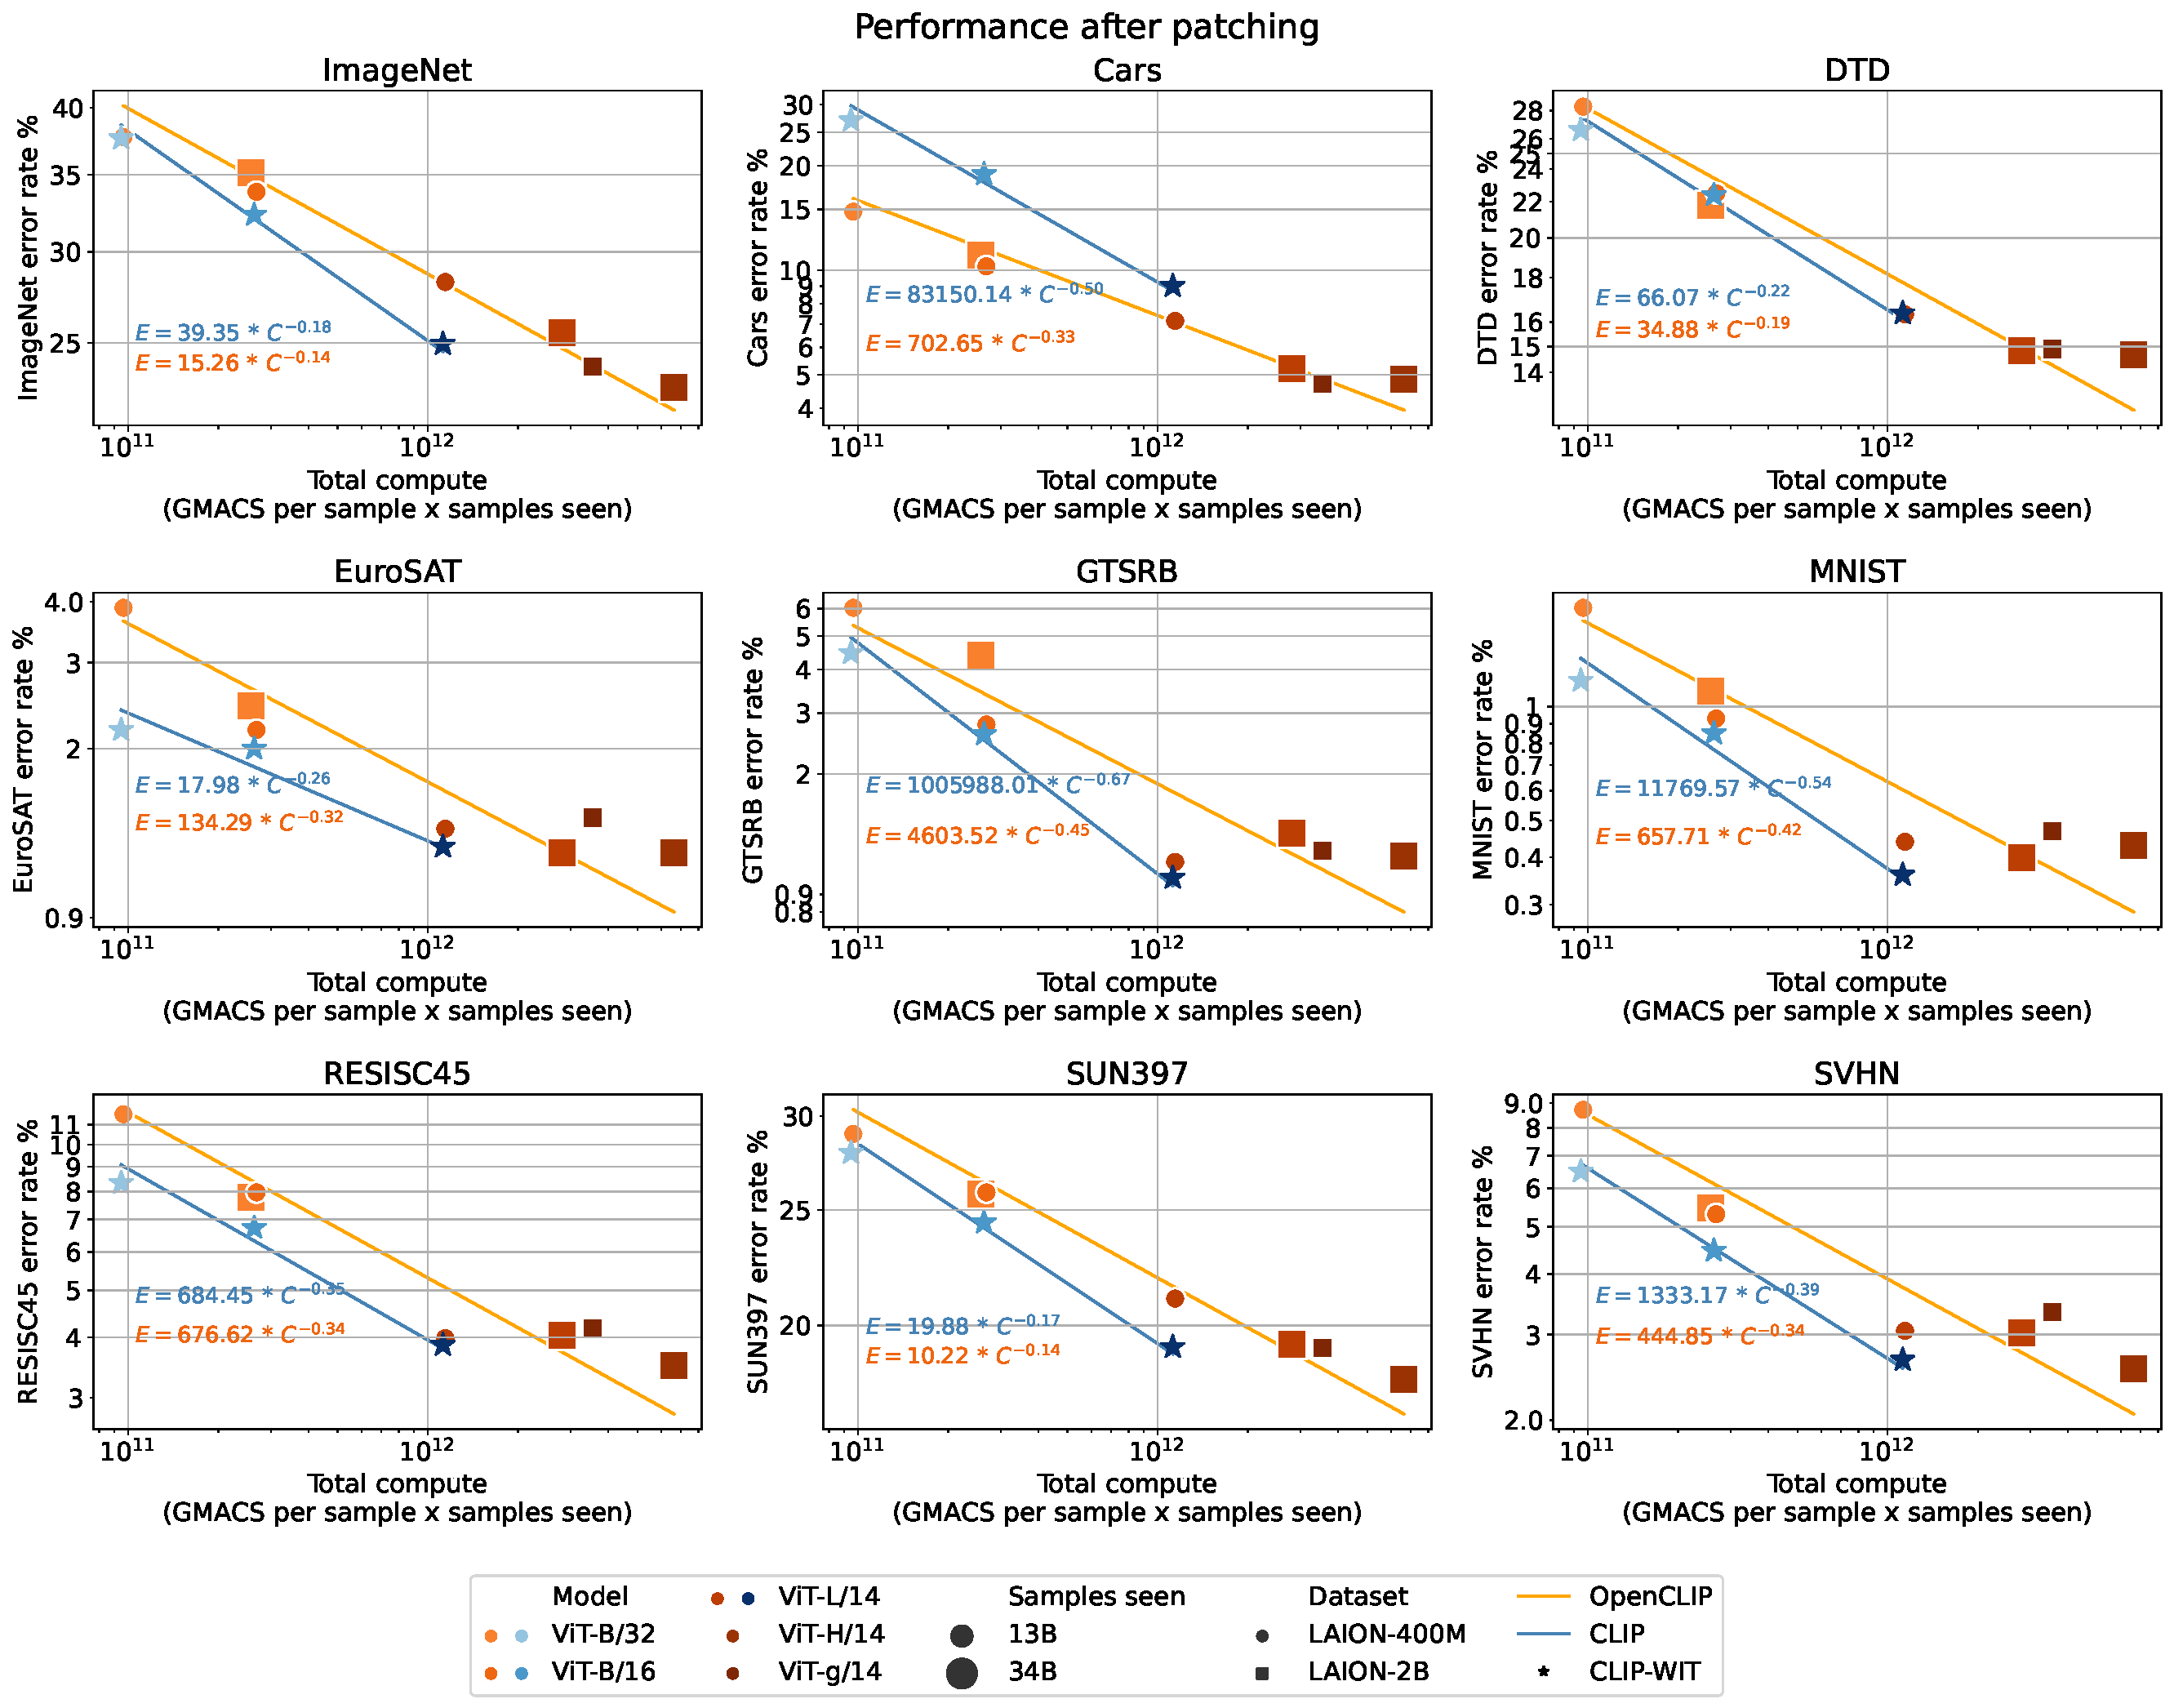
\includegraphics[width=\linewidth]{images/scaling_breakdown_patch.pdf}
    \caption{Scaling trends of patched models \cite{ilharco2022patching}, on ImageNet and eight other downstream tasks used for the fine-tuning experiments in Section \ref{subsect:scaling_laws_finetune}.}
    \label{fig:ft-eight-patch}
\end{figure}

\begin{table}
\footnotesize
\centering
\rowcolors{2}{light-light-gray}{white}
\begin{tabular}{lllrrrrrrr}
\toprule
& & & &  \multicolumn{3}{c}{ImageNet} & \multicolumn{3}{c}{CIFAR100} \\
 Model & Samples Seen & Dataset & VTAB & 10 shot & 25 shot & Full & 10 shot & 25 shot & Full \\
\midrule

           ViT-B/32 &                 13B &         CLIP-WIT &    69.71 &                          59.16 &                          65.27 &                          75.61 &             63.93 &             70.64 &             79.97 \\
           ViT-B/32 &                 13B &       LAION-400M &    71.84 &                          59.36 &                          65.17 &                          74.90 &             70.50 &             75.18 &             82.92 \\
%          ViT-B/32 &                 34B &         LAION-2B &    71.43 &                          61.89 &                          67.49 &                          76.60 &             74.24 &             78.73 &             85.06 \\
           ViT-B/32 &                 34B &         LAION-2B &    71.53 &                          62.40 &                          67.98 &                          76.93 &             75.47 &             79.97 &             85.99 \\
          ViT-B/16 &                 13B &         CLIP-WIT &    71.25 &                          65.42 &                          70.97 &                          79.82 &             68.91 &             74.67 &             82.40 \\
           ViT-B/16 &                 13B &       LAION-400M &    72.72 &                          64.46 &                          69.94 &                          78.74 &             71.96 &             77.21 &             84.07 \\
           ViT-L/14 &                 13B &         CLIP-WIT &    73.77 &                          73.51 &                          77.67 &                          84.39 &             77.57 &             81.91 &             87.14 \\
           ViT-L/14 &                 13B &       LAION-400M &    73.98 &                          70.86 &                          75.02 &                          81.77 &             78.06 &             82.48 &             87.95 \\
           ViT-L/14 &                 34B &         LAION-2B &    74.48 &                          73.94 &                          77.45 &                          83.46 &             82.76 &             86.04 &             90.14 \\
           ViT-H/14 &                 34B &         LAION-2B &    \textbf{75.96} &                          \textbf{75.79} &                          \textbf{79.07} &                          \textbf{84.85} &             \textbf{84.74} &             \textbf{87.82} &             \textbf{91.43} \\
           ViT-g/14 &                 13B &         LAION-2B &    75.18 &                          74.87 &                          78.25 &                          84.09 &             84.66 &             87.76 &             91.09 \\
\bottomrule
\end{tabular}
\caption{
Scaling model and data size leads to lower error linear classifers on ImageNet~\cite{Deng2009a}, CIFAR100~\cite{Krizhevsky2009}, and the visual task adaptation benchmark (VTAB)~\cite{zhai2019large}.
     We train linear probes for models with at least 13B samples seen.
     We train probes by first caching the image features, thus no data augmentation is used.
     $k$ shot denotes that $k$ images per-class are used to train the linear probe.
     }
    \label{tab:lp}
\end{table}

\begin{table}
\scriptsize
\centering
\setlength\tabcolsep{3pt}
\rowcolors{2}{light-light-gray}{white}
\begin{tabular}{lrlrrrrrrrrr}     
\toprule                           

& & & \multicolumn{9}{c}{Top-1 Accuracy (\%)} \\
Arch. & \# samples &  Dataset & ImageNet & Cars & DTD & EuroSAT & GTSRB & MNIST & RESISC45 & SUN397 & SVHN \\                                   
\midrule                                                                                                                                                                           ViT-B/32 &          13B &    CLIP-WIT &         63.35 &     59.73 &    43.99 &        45.81 &      32.56 &      48.25 &         60.65 &       63.18 &     31.61 \\                                  
 ViT-B/32 &          13B &  LAION-400M &         62.94 &     79.24 &    54.47 &        50.89 &      41.98 &      37.44 &         57.62 &       66.28 &     30.36 \\                                  
ViT-B/32 &          34B &    LAION-2B &         65.63 &     84.45 &    54.04 &        47.22 &      36.48 &      63.34 &         67.70 &       67.94 &     41.66 \\                                   
ViT-B/16 &          13B &    CLIP-WIT &         68.33 &     64.61 &    45.11 &        53.96 &      43.34 &      51.80 &         65.76 &       65.50 &     51.98 \\                                  
ViT-B/16 &          13B &  LAION-400M &         67.05 &     83.63 &    51.01 &        49.15 &      43.45 &      66.29 &         64.97 &       67.96 &     34.12 \\          

ViT-L/14 &          13B &    CLIP-WIT &         75.54 &     77.75 &    55.32 &        60.22 &      50.55 &      \textbf{76.36} &         71.05 &       68.28 &     \textbf{58.45} \\                                  
ViT-L/14 &          13B &  LAION-400M &         72.75 &     89.53 &    60.16 &        61.48 &      49.89 &      76.09 &         68.92 &       71.44 &     49.54 \\                                  
ViT-L/14 &          34B &    LAION-2B &         75.26 &     92.71 &    62.82 &        64.44 &      56.14 &      54.10 &         73.25 &       73.56 &     40.84 \\      ViT-H/14 &          34B &    LAION-2B &         \textbf{77.95} &     \textbf{93.50} &    67.50 &        \textbf{71.04} &      \textbf{58.35} &      72.83 &         \textbf{75.87} &       75.23 &     52.51 \\                           
ViT-g/14 &          13B &    LAION-2B &         76.66 &     92.90 &    \textbf{68.24} &        62.70 &      49.87 &      68.46 &         74.57 &       \textbf{75.24} &     39.34 \\                                 
\bottomrule
\end{tabular}
\caption{
    Zero-shot accuracy for various models on downstream tasks from Section \ref{sec:appendix:finetuning}.
    \label{tab:appendix:joint_ft_zs}
    }
\end{table}




\begin{table}
\scriptsize
\centering
\setlength\tabcolsep{5pt}
\rowcolors{2}{light-light-gray}{white}
\begin{tabular}{lrlrrrrrrrr}     
\toprule                           

& & & \multicolumn{8}{c}{Top-1 Accuracy (\%)} \\
Arch. & \# samples &  Dataset & Cars & DTD & EuroSAT & GTSRB & MNIST & RESISC45 & SUN397 & SVHN \\                                      
\midrule                                                                                    ViT-B/32 &          13B &    CLIP-WIT &     72.19 &    79.04 &        98.37 &      98.19 &      99.36 &         93.62 &       73.57 &     95.33 \\                                                  
 ViT-B/32 &          13B &  LAION-400M &     84.14 &    78.99 &        97.96 &      98.37 &      99.55 &         93.54 &       72.76 &     95.67 \\                                                  
 ViT-B/32 &          34B &    LAION-2B &     88.16 &    81.01 &        97.96 &      98.00 &      99.34 &         94.46 &       75.04 &     95.46 \\                             ViT-B/16 &          13B &    CLIP-WIT &     83.10 &    82.45 &        98.26 &      98.84 &      99.44 &         94.90 &       76.94 &     96.33 \\                                                  
ViT-B/16 &          13B &  LAION-400M &     89.22 &    82.34 &        98.22 &      98.82 &      99.54 &         94.67 &       75.81 &     96.18 \\                                                                      
ViT-L/14 &          13B &    CLIP-WIT &     90.87 &    84.63 &        98.78 &      \textbf{99.18} &     99.59 &         96.33 &       81.22 &     \textbf{97.42} \\                                                  
 ViT-L/14 &          13B &  LAION-400M &     92.35 &    84.31 &        98.56 &      99.01 &      99.62 &         96.05 &       79.08 &     96.97 \\                                                  
 ViT-L/14 &          34B &    LAION-2B &     94.42 &    \textbf{85.69} &        \textbf{98.85} &      98.92 &      \textbf{99.67} &         96.06 &       81.10 &     97.06 \\
  ViT-H/14 &          34B &    LAION-2B &     94.80 &    85.32 &        \textbf{98.85} &      99.03 &      99.55 &         \textbf{96.52} &       \textbf{82.08} &     97.40 \\                                                  
 ViT-g/14 &          13B &    LAION-2B &     \textbf{94.84} &    85.48 &        98.44 &      98.95 &      99.54 &         95.95 &       80.82 &     96.67 \\                          
\bottomrule
\end{tabular}
\caption{
    Accuracy after fine-tuning for various models on downstream tasks from Section \ref{sec:appendix:finetuning}. We fine-tune jointly on the eight downstream image classification tasks, alternating batches from each task.
    We fine-tune only the parameters of the vision encoder, using a fixed classification head for each task initialized with the weights from the zero-shot model.
    \label{tab:appendix:joint_ft_ft}
    }
\end{table}

\begin{table}
\scriptsize
\centering
\setlength\tabcolsep{3pt}
\rowcolors{2}{light-light-gray}{white}
\begin{tabular}{lrlrrrrrrrrr}     
\toprule                           

& & & \multicolumn{9}{c}{Top-1 Accuracy (\%)} \\
Arch. & \# samples &  Dataset & ImageNet & Cars & DTD & EuroSAT & GTSRB & MNIST & RESISC45 & SUN397 & SVHN \\                                                    
\midrule                                                                                 ViT-B/32 &          13B &    CLIP-WIT &         62.36 &     72.96 &    73.40 &        97.81 &      95.53 &      98.83 &         91.67 &       72.08 &     93.50 \\
ViT-B/32 &          13B &  LAION-400M &         62.27 &     85.24 &    71.70 &        96.11 &      93.97 &      98.18 &         88.44 &       71.03 &     91.29 \\
ViT-B/32 &          34B &    LAION-2B &         64.84 &     88.93 &    78.19 &        97.56 &      95.60 &      98.90 &         92.21 &       74.22 &     94.53 \\
ViT-B/16 &          13B &    CLIP-WIT &         67.70 &     81.07 &    77.61 &        98.00 &      97.40 &      99.15 &         93.27 &       75.59 &     95.53 \\
ViT-B/16 &          13B &  LAION-400M &         66.18 &     89.73 &    77.50 &        97.81 &      97.22 &      99.07 &         92.03 &       74.13 &     94.69 \\
ViT-L/14 &          13B &    CLIP-WIT &         75.04 &     90.98 &    83.62 &        98.74 &      \textbf{98.99} &      \textbf{99.64} &         96.14 &       80.81 &     97.34 \\
ViT-L/14 &          13B &  LAION-400M &         71.76 &     92.85 &    83.67 &        98.63 &      98.88 &      99.56 &         96.02 &       78.93 &     96.95 \\
ViT-L/14 &          34B &    LAION-2B &         74.50 &     94.79 &    85.16 &        \textbf{98.78} &      98.65 &      99.60 &         95.97 &       80.72 &     96.98 \\
ViT-H/14 &          34B &    LAION-2B &         \textbf{77.12} &     95.15 &    \textbf{85.32} &        \textbf{98.78} &      98.84 &      99.57 &         \textbf{96.51} &       \textbf{81.98} &     \textbf{97.45} \\
ViT-g/14 &          13B &    LAION-2B &         76.16 &     \textbf{95.27} &    85.11 &        98.56 &      98.80 &      99.53 &         95.83 &       80.86 &     96.66 \\        
\bottomrule
\end{tabular}
\caption{
    Accuracy after joint patching \cite{ilharco2022patching} for various models on downstream tasks from Section \ref{sec:appendix:finetuning}. Patching by jointly fine-tuning on the eight tasks with the exception of ImageNet (used only as control), then interpolating the weights of the fine-tuned model with the weights of the zero-shot model. The mixing coefficient for the interpolation is chosen so it maximizes average accuracy on the eight downstream tasks while maintaining ImageNet accuracy within 1 percentage point of the corresponding zero-shot model.
    \label{tab:appendix:joint_ft_patch}
    }
\end{table}


\begin{table}
\scriptsize
\centering
\setlength\tabcolsep{2.5pt}
\rowcolors{2}{light-light-gray}{white}

\begin{tabular}{llllrrrrrrrrr}
\toprule
         & & & & & & & \multicolumn{6}{c}{Top-1 Accuracy (\%)} \\
   Model & Im Size &  Dataset & Extra FT & Params (M) & GMAC & Acts (M) &                 IN & IN-ReaL & IN-V2 &  IN-A &  IN-R & IN-Sketch \\
\midrule
ViT-B/32 &     224 & CLIP-WIT &     None &       88.2 &   4.4 &      5.0 &              81.93 &   87.17 & 70.70 & 22.57 & 55.90 &     45.04 \\
ViT-B/32 &     224 & LAION-2B &     None &       88.2 &   4.4 &      5.0 &              82.58 &   87.54 & 71.21 & 22.85 & 59.16 &     49.07 \\
ViT-B/32 &     224 & LAION-2B &   IN-12k &       88.2 &   4.4 &      5.0 &              83.30 &   87.81 & 72.50 & 30.57 & 57.06 &     45.74 \\
ViT-B/32 &     384 & CLIP-WIT &   IN-12k &       88.3 &  13.1 &     16.5 &              85.11 &   89.04 & 74.53 & 44.75 & 58.21 &     45.75 \\
ViT-B/16 &     224 & CLIP-WIT &     None &       86.6 &  17.6 &     23.9 &              85.28 &   89.16 & 75.57 & 47.23 & 66.02 &     50.94 \\
ViT-B/32 &     384 & LAION-2B &   IN-12k &       88.3 &  13.1 &     16.5 &              85.38 &   89.20 & 75.08 & 47.95 & 60.37 &     47.95 \\
ViT-B/16 &     224 & LAION-2B &     None &       86.6 &  17.6 &     23.9 &              85.47 &   89.43 & 75.13 & 41.57 & 68.75 &     55.40 \\
ViT-B/16 &     384 & CLIP-WIT &     None &       86.9 &  55.5 &    101.6 &              86.24 &   89.71 & 76.68 & 57.55 & 67.22 &     52.15 \\
ViT-B/16 &     384 & LAION-2B &     None &       86.9 &  55.5 &    101.6 &              86.53 &   90.04 & 77.55 & 56.96 & 69.94 &     55.85 \\
ViT-B/16 &     384 & LAION-2B &   IN-12k &       86.9 &  55.5 &    101.6 &              87.17 &   90.11 & 78.16 & 62.61 & 65.53 &     52.62 \\
ViT-L/14 &     224 & LAION-2B &     None &      304.2 &  81.1 &     88.8 &              87.30 &   90.10 & 78.42 & 59.89 & 81.70 &     64.81 \\
ViT-H/14 &     224 & LAION-2B &     None &      632.0 & 167.4 &    139.4 &              87.59 &   90.17 & 79.36 & 65.56 & \textbf{83.28} &     \textbf{67.41} \\
ViT-L/14 &     336 & LAION-2B &     None &      304.5 & 191.1 &    270.2 &              87.78 &   90.30 & 79.07 & 69.03 & 82.60 &     64.79 \\
ViT-L/14 &     224 & CLIP-WIT &     None &      304.2 &  81.1 &     88.8 &              87.85 &   90.31 & \textbf{79.59} & 71.79 & 82.32 &     62.63 \\
ViT-L/14 &     224 & LAION-2B &   IN-12k &      304.2 &  81.1 &     88.8 &              87.89 &   90.30 & 78.51 & 67.01 & 78.26 &     62.06 \\
ViT-L/14 &     336 & LAION-2B &   IN-12k &      304.5 & 191.1 &    270.2 &              88.17 &   90.43 & 78.84 & 73.64 & 77.68 &     60.97 \\
ViT-L/14 &     224 & CLIP-WIT &   IN-12k &      304.2 &  81.1 &     88.8 &              88.17 &   90.37 & 79.38 & 72.33 & 78.68 &     61.40 \\
ViT-H/14 &     224 & LAION-2B &   IN-12k &      632.0 & 167.4 &    139.4 &              88.25 &   90.41 & 79.22 & 70.72 & 82.82 &     65.32 \\
ViT-H/14 &     336 & LAION-2B &   IN-12k &      632.5 & 391.0 &    407.5 &              \textbf{88.50} &   \textbf{90.49} & 79.55 & \textbf{75.68} & 82.26 &     64.62 \\
\bottomrule
\end{tabular}
\caption{Fine-tune results for ImageNet-1k and associated robustness test sets (ImageNet-ReaL~\citep{beyer2020we}, ImageNet-V2~\citep{pmlr-v97-recht19a}, ImageNet-A~\citep{imageneta}, Imagenet-R~\citep{imagenetr}, and ImageNet-Sketch~\citep{imagenetsketch}). Rows with the 'Extra FT' set to IN-12k were fine-tuned on a 12k class subset of ImageNet-22k before fine-tuning on ImageNet.}
\label{table:finetune_results}
\end{table}


\begin{table}
\footnotesize
\centering
\rowcolors{2}{light-light-gray}{white}
\begin{tabular}{lllll}
\toprule
        Hyperparameter &                B/32 &                B/16 &                L/14 &                H/14 \\
\midrule
    Peak Learning-rate &            1.00E-03 &            3.00E-04 &            6.00E-05 &            5.00E-05 \\
            Batch Size &                4096 &                2048 &                2048 &                2048 \\
                Epochs &                  50 &                  50 &                  50 &                  50 \\
         Warmup Epochs &                  10 &                  10 &                  10 &                  10 \\
   Layer-wise LR Decay &                0.65 &                 0.7 &                 0.8 &                0.82 \\
  EMA Weight Smoothing &              0.9998 &              0.9998 &              0.9997 &              0.9998 \\
          Weight Decay &                0.05 &                0.05 &                0.01 &                0.02 \\
       Label Smoothing &                 0.1 &                 0.1 &                 0.1 &                 0.1 \\
          Stoch. Depth &                 0.1 &                 0.1 &                 0.2 &                 0.2 \\
               Dropout &                   0 &                   0 &                   0 &                   0 \\
     Gradient Clipping &                   3 &                   3 &                   3 &                   2 \\
Rand Augment (Uniform) &      M=U(0, 8), N=2 &      M=U(0, 9), N=2 &      M=U(0, 9), N=3 &     M=U(0, 8), N=4  \\
     Random Erase Prob &                 0.3 &                 0.3 &                 0.3 &                 0.3 \\
     Random Resize Crop &                 Yes &                 Yes &                 Yes &                Yes \\
           Mixup Alpha &                   0 &                   0 &                   0 &                   0 \\
          Cutmix Alpha &                   0 &                   0 &                   0 &                   0 \\
          Color Jitter &                   0 &                   0 &                   0 &                   0 \\
\bottomrule
\end{tabular}
\caption{ImageNet fine-tune hyper-parameters.}
\label{table:imagenet_ft_hparam}
\end{table}

\begin{table}
\footnotesize
\centering
\rowcolors{2}{light-light-gray}{white}
\begin{tabular}{lllll}
\toprule
        Hyperparameter &           B/32 &           B/16 &           L/14 &           H/14 \\
\midrule
    Peak Learning-rate &       1.00E-03 &       5.00E-04 &       5.00E-04 &       4.00E-04 \\
            Batch Size &           4096 &           4096 &           4096 &           4096 \\
                Epochs &             60 &             60 &             60 &             60 \\
         Warmup Epochs &             10 &             10 &             10 &             10 \\
   Layer-wise LR Decay &           0.65 &            0.7 &            0.8 &           0.86 \\
  EMA Weight Smoothing &         0.9998 &         0.9998 &         0.9999 &         0.9999 \\
          Weight Decay &           0.05 &           0.05 &           0.02 &           0.02 \\
       Label Smoothing &            0.1 &            0.1 &            0.1 &            0.1 \\
          Stoch. Depth &            0.1 &            0.1 &            0.2 &            0.2 \\
               Dropout &              0 &              0 &              0 &              0 \\
     Gradient Clipping &              3 &              3 &              3 &              2 \\
Rand Augment (Uniform) & M=U(0, 8), N=2 & M=U(0, 8), N=2 & M=U(0, 9), N=2 & M=U(0, 8), N=3 \\
     Random Erase Prob &            0.3 &            0.3 &            0.3 &            0.3 \\
    Random Resize Crop &            Yes &            Yes &            Yes &            Yes \\
           Mixup Alpha &              0 &              0 &              0 &              0 \\
          Cutmix Alpha &              0 &              0 &              0 &              0 \\
          Color Jitter &              0 &              0 &              0 &              0 \\
\bottomrule
\end{tabular}
\caption{ImageNet-12k intermediate fine-tune hyper-parameters.}
\label{table:imagenet_ft12k_hparam}
\end{table}


\subsubsection{Control experiments}
\label{sec:appendix:control_exp}

\textbf{Batch size during pre-training.} To be able to train efficiently on a large number of GPUs (up to 1520 in this work), it is desired to maximize the local batch size for each GPU worker for performing data parallel distributed training. For this large amount of GPUs, it leads to training with global batch sizes of 86K-88K. As we would like to also re-use experiments that were already performed with smaller batch sizes of 32K-45K, we execute control experiments to reassure that varying batch size in those ranges does not alter observed model performance on downstream tasks strongly. The experiments summarized in Table~\ref{tab:batch_size} provide evidence that performance variation due to changes in batch size is small, in the range of $0.2-0.5\%$ across different settings, which is small enough not to distort the trends  observed in the effect of scale, where the changes are substantially larger.


\begin{table}[!htb]
\setlength\tabcolsep{3.0pt}
    \centering
    \small
    \begin{tabular}{lcc}\toprule
       Batch size /  & 32k/38k (L/14) & 64k (B/16) / \\
      Model & & 86k (+lr tune) \\ \midrule
    ViT B/32 & 62.9 & 63.37 \\
    %\midrule
%    Ours & LAION-400M & L/14 &  &  &  \\
    ViT B/16 & 67.34 & 67.86 \\
    ViT L/14 & 72.8 & 72.98 \\\bottomrule
    \end{tabular}
    \caption{
    Batch size control experiments, zero-shot ImageNet top-1 accuracy. Executed on LAION-400M, 13B samples seen (32 full epochs).
    \vspace{-1em}
    }
    \label{tab:batch_size}
\end{table}

% Testing dependence of performance on batch size during pre-training.

% The main difference in training recipes is the batch size due to different compute environments, and our experiments with varying batch sizes suggest that the batch size changes do not explain the change in scaling trends.

% Compared to the original CLIP training procedure\citep{radford2021learning}, we work with larger batch sizes and adapt the learning rate accordingly.
%We opt for larger batch sizes to allow for more efficient distributed training; maximizing the local batch size per GPU and using close to one thousand GPUs lead us to global batch sizes in the range of 86-88K samples.
% In order to assess the validity of re-using measurements obtained with different batch sizes, we perform a number of control experiments varying batch size from 32K to 86-88K, and observe a difference of $0.2-0.5\%$ across different settings (see Appendix Sec. \ref{sec:appendix:control_exp}), which is small enough not to confound observations on the effect of scale.


\textbf{LAION-400M and 400M subset of LAION-2B size.} For 400M data scale, we are using LAION-400M dataset, as it was already validated by numerous previous works. This is not a subset of LAION-2B, as both were obtained by the same, but separately executed composition procedure using Common Crawl. To test that LAION-400M and LAION-2B can be considered as two different scale of the same data distribution, we extracted a random 400M subset from LAION-2B and conducted a pre-training experiment using our reference OpenCLIP ViT-B/32 model, 13B samples seen scale. We evaluated the pre-trained model on ImageNet zero-shot classification task, comparing it to same model pre-trained on LAION-400M. The outcome shows no significant difference between the performance of both models. This provides evidence that LAION-400M is comparable to a 400M subset extracted from LAION-2B, and can be thus considered to be a smaller scale of same data distribution.

\begin{table}[!htb]
\setlength\tabcolsep{4.0pt}
    \centering
    \small
    \begin{tabular}{lcc}\toprule
    Model/Dataset & 400M LAION-2B subset &  LAION-400M \\ \midrule
    ViT B/32 & 63.56 & 63.37 \\\bottomrule
    \end{tabular}
    \caption{
    400M data scale subset control experiments, zero-shot ImageNet top-1 accuracy. Executed either on 400M subset of LAION-2B or on LAION-400M, 13B samples seen (32 full epochs).
    \vspace{-1em}
    }
    \label{tab:subset_400M}
\end{table}

\textbf{Pre-training trial-to-trial variance.} To have a sanity check of trial-to-trial variance for model pre-training, we trained our reference ViT-B/32 model, 13B samples seen scale, for two trials using exactly the same hyper-parameters (lr=$0.001$, batch size 86K, warm up 2K). We evaluated the two trials on ImageNet zero-shot classification task. The result suggests a small variance of around 0.1\%, which is much smaller than variations observed when changing the scales. This allows us to conclude that scaling trends we observe are not distorted by variance caused by trial-to-trial pre-training.   
\begin{table}[!htb]
\setlength\tabcolsep{3.0pt}
    \centering
    \small
    \begin{tabular}{lcc}\toprule
       Trial  & ImageNet zero-shot top-1  \\ \midrule
        1 & 63.28 \\
        2 & 63.67 \\\bottomrule
    \end{tabular}
    \caption{
    Trial-to-trial variance control experiment. Executed on LAION-400M, 13B samples seen (32 full epochs) using ViT B/32 model.
    \vspace{-1em}
    }
    \label{tab:trial_to_trial}
\end{table}

\textbf{Resampling vs full shuffled training.} During our larger scale pre-training experiments featuring LAION-2B, it became important to allow for frequent checkpoint saving. Saving within a running epoch would require to memorize which samples were already seen, to be able to resume training in such a way that only previously not seen samples would be taken. To simplify the procedure, we have tested a version that does not perform epoch-wise training, taking a pre-defined number of samples instead for a virtual "step" through data. Such a resampling procedure can have repeated samples in the subset of data that contains in total the number of samples equal to number of samples in one full epoch through the dataset. As such training procedure differs from standard epoch-wise training, we conducted test experiments to check whether this results in differences in performance of pre-trained models when comparing to standard epoch-wise shuffling training. We trained our reference ViT-B/32 model and ViT-B/16 model on LAION-400M either using standard epoch-wise training with shuffling or the training that involves described resampling procedure. We observed only negligible differences of 0.1\%-0.3\%, concluding that using simple resampling cannot distort scaling trends observed in the study. 

\begin{table}[!htb]
\setlength\tabcolsep{3.0pt}
    \centering
    \small
    \begin{tabular}{lcc}\toprule
    Model & Resampling &  Full shuffling \\ \midrule
    ViT B/32 & 63.37 & 63.28; 63.67 \\\bottomrule
    \end{tabular}
    \caption{
    Resampling vs. full shuffling control experiments, zero-shot ImageNet top-1 accuracy. Executed on LAION-400M, 13B samples seen (32 full epochs).
    \vspace{-1em}
    }
    \label{tab:resampling_shuffling}
\end{table}

% corresponding to the number of samples that equals number of samples in 1 epoch through the dataset.

\subsubsection{Further detailed results and analysis}
\label{sec:appendix:further_results}

\begin{table}[!tbh]
\centering
\small
\rowcolors{2}{light-light-gray}{white}
%\setlength{\tabcolsep}{2pt}
%\resizebox{\linewidth}{!}{
\begin{tabular}{@{}lclll@{}}
\toprule
\textbf{Model}                     & \textbf{Samples seen} & \textbf{LAION-80M} & \textbf{LAION-400M} & \textbf{LAION-2B} \\ \midrule
\textbf{ViT-B/32} & 3B           & 38.05     & 41.53      & 43.66       \\
                          & 13B          & 42.30     & 46.18       & 45.50       \\
                          & 34B          & 42.10         & 46.41      &50.69        \\ \midrule
\textbf{ViT-B/16} & 3B           & 43.48     & 45.14      & 46.93       \\
                          & 13B          & 44.42     & 48.39       & 48.72       \\
                          & 34B          & 44.45         & 48.31      & 52.60        \\ \midrule                          
\textbf{ViT-L/14} & 3B           & 45.69     & 50.50      & 51.64       \\         
& 13B          & 46.36         & 51.51      & 53.01           \\
                          & 34B          & 45.70         & 52.83       & 54.63       \\ \midrule 
\textbf{ViT-H/14} & 34B           & -     & -      & 56.43       \\         \midrule 
\textbf{ViT-g/14} & 13B           & -     & -      & 56.54       \\         \bottomrule 

\end{tabular}


%}
\caption{Detailed results on VTAB+~\cite{Schuhmann2022} zero-shot classification, where we average over 35 tasks. 
}
\label{table:zeroshot_vtab_plus}
\end{table}

%TODO: here extended large tables with full details belong (eg VTAB+ full table as in NeurIPS paper) (DONE)

\begin{table}[ht]
\centering
\small
\rowcolors{2}{light-light-gray}{white}
\begin{tabular}{@{}lcccccc@{}}
\toprule
Dataset & B/32 (34B)&B/16 (34B)&L/14 (34B)&g/14 (13B)&H/14 (34B)\\  \midrule
INet & 66.47 &70.22 &75.20 &76.66 &\textbf{77.97 }\\
INet-v2 & 58.16 &62.28 &67.69 &69.61 &\textbf{70.82 }\\
INet-R & 76.47 &80.59 &87.41 &88.65 &\textbf{89.32 }\\
INet-S & 53.72 &56.09 &63.28 &65.22 &\textbf{66.57 }\\
ObjNet & 48.78 &56.05 &65.50 &67.47 &\textbf{69.70 }\\
INet-A & 25.43 &38.23 &53.88 &57.11 &\textbf{59.23 }\\
CIFAR-10 & 93.65 &94.94 &96.64 &97.05 &\textbf{97.42 }\\
CIFAR-100 & 75.47 &76.83 &83.36 &83.91 &\textbf{84.68 }\\
MNIST & 67.73 &65.99 &54.87 &69.04 &\textbf{72.94 }\\
Flowers102 & 72.35 &71.23 &75.90 &77.61 &\textbf{80.21 }\\
Cars & 86.15 &88.50 &92.61 &92.77 &\textbf{93.46 }\\
SVHN & 43.51 &51.39 &46.30 &\textbf{60.33 }&56.13 \\
FER2013 & 46.02 &51.78 &\textbf{53.71 }&46.57 &51.76 \\
RenderedSST2 & 57.17 &59.80 &59.31 &\textbf{64.58 }&64.09 \\
Pets & 89.81 &90.52 &93.21 &94.28 &\textbf{94.39 }\\
Caltech-101 & 83.50 &83.83 &85.04 &\textbf{85.22 }&85.04 \\
VOC2007-Cl & 79.75 &78.85 &80.52 &\textbf{81.03 }&77.61 \\
SUN397 & 68.57 &70.85 &74.33 &\textbf{75.40 }&75.22 \\
FGVC Aircraft & 24.06 &27.00 &36.93 &37.80 &\textbf{42.75 }\\
Country211 & 16.78 &20.31 &26.36 &28.73 &\textbf{30.01 }\\
DTD & 55.64 &56.33 &62.77 &\textbf{68.14 }&67.87 \\
GTSRB & 49.49 &48.24 &56.10 &49.74 &\textbf{58.45 }\\
STL10 & 96.55 &97.86 &\textbf{98.86 }&98.59 &98.44 \\
Retino & \textbf{73.42 }&67.96 &21.06 &43.42 &23.80 \\
EuroSAT & 46.94 &53.46 &65.15 &64.80 &\textbf{71.74 }\\
RESISC45 & 60.71 &62.76 &66.67 &\textbf{71.71 }&69.57 \\
PCAM & \textbf{59.44 }&56.37 &55.26 &55.09 &53.63 \\
CLEVR Counts & 15.02 &21.49 &31.09 &\textbf{33.19 }&27.84 \\
CLEVR Dist & 14.54 &\textbf{21.07 }&16.10 &17.73 &16.77 \\
DSPRITES Orient & \textbf{3.77 }&2.68 &2.00 &3.08 &2.61 \\
DSPRITES pos & 2.80 &3.30 &3.15 &\textbf{3.54 }&3.14 \\
SmallNORB Elv & \textbf{11.70 }&11.30 &10.95 &11.34 &11.13 \\
SmallNORB Azim & 5.86 &5.67 &5.63 &\textbf{5.88 }&5.50 \\
DMLAB & 17.48 &19.93 &\textbf{22.43 }&19.02 &14.20 \\
KITTI Dist & \textbf{27.14 }&17.16 &22.93 &14.63 &11.11 \\

\midrule
\textbf{VTAB+ (Avg.)} & 50.69 &52.60 &54.63 &\textbf{56.54} &56.43 \\
\bottomrule
\end{tabular}
\caption{Detailed zero-shot top-1 classification results of LAION-2B models on VTAB+ 35 tasks. We highlight the best results for each downstream dataset.}
\label{table:vtab_plus_details}
\end{table}

\textbf{Consistency of scaling trends for CLIP and openCLIP}

In Fig.~\ref{fig:resnet_scaling_trends}, we complement the results we found in Fig.~\ref{fig:fig1} and  show scaling trends with additional ResNet models from OpenAI trained on the WebImageText (WIT) dataset. Despite different model architectures, we see the same consistent pattern - both OpenAI’s ResNets and ViT trained on WIT demonstrate stronger scaling on zero-shot classification but worse scaling on retrieval than openCLIP trained on LAION datasets.


\textbf{Details of zero-shot classification results.} Complementing results from the Section \ref{subsect:scaling_laws}, we provide summary tables for the performance measure on different downstream tasks:  ImageNet (Tab.~\ref{table:zeroshot_im1k}), ImageNet robustness(Tab.~\ref{table:zeroshot_imrobustness}), MS-COCO image retrieval (Tab.~\ref{table:zeroshot_mscoco_image_retrieval}) and text retrieval (Tab.~\ref{table:zeroshot_mscoco_text_retrieval}), Flickr30K image retrieval (Tab.~\ref{table:zeroshot_flickr30k_image_retrieval}) and text retrieval (Tab.~\ref{table:zeroshot_flickr30k_text_retrieval}), and VTAB+ (Tab.~\ref{table:zeroshot_vtab_plus} and ~\ref{table:vtab_plus_details}).

\textbf{Details of linear probing results}. To supplement Figures~\ref{fig:lp1} and \ref{fig:lp2}, we provide the corresponding Table~\ref{tab:lp} with detailed results.

%\textbf{Details of fine-tuning results}. To supplement Figure, we provide the corresponding Tablw~\ref{table:fi} with full details.
%ToDO: GMAC for architecture hyperparam table (DONE)

%TODO: full table on model/data/sample seen scales for zero shot im1k (DONE)

%ToDo : full table on model/data/sample seen scales for zero shot retrieval  (Flickr30k) (DONE)

%ToDo Mehdi, Romain, Ross, Jenia: table on training hyperparams. Table \ref{table:openclip_hyper_parameters}. Introduce samples seen, and GPU-hours (DONE)

\textbf{Architecture and training hyperparameters.} We provide overview for architecture (Tab.~\ref{table:openclip_architectures}) and pre-training hyper-parameters (Tab.~\ref{table:openclip_hyper_parameters}) that we have used in the experiments. 

\begin{table}[ht]
\centering
\setlength\tabcolsep{5pt}
\footnotesize
\rowcolors{2}{light-light-gray}{white}
\begin{tabular}{@{}llrrrrrrr@{}}
\toprule
\textbf{Model} & \textbf{Dataset} & \textbf{BS. (global)} & \textbf{LR.} & \textbf{Warm.} & \textbf{\#samples}. &  \textbf{\#GPUs} & \textbf{Time (hrs.)} & \textbf{GPU-h}/\textbf{MWh} \\ \midrule
%B/32 (400M)                & 256 (32768)   & $5\text{e-}4$          & 2K         & 32   & 128 & 36          & 4608         \\
%B/32 (2B)                  & 416 (46592)   & $5.5\text{e-}4$        & 10K        & 16   & 112    & 210      &  23520          \\
%B/16 (400M)                & 192 (33792)   & $5\text{e-}4$          & 2K         & 32   & 176  & 61 &    10736               \\
%L/14 (400M)                & 96 (38400)    & $6\text{e-}4$          & 5K         & 32  & 400 & 88   &     35200             \\ \bottomrule
%L/14 (2B)                  & 224 (8601)         & 384    & $1\text{e-}3$          & 10K        & 16     & 88                     \\ \bottomrule
B/32 & LAION-80M & 256(32768) & 5e-4 & 2K & 3B & 128 & 7 & 836/0.29 \\
B/32 & LAION-80M & 256(32768) & 5e-4 & 2K & 13B & 128 & 33 & 4181/1.46 \\
B/32 & LAION-80M & 256(88064) & 1e-3 & 10K & 34B & 344 & 96 & 32953/11.53 \\
B/32 & LAION-400M & 256(88064) & 1e-3 & 10K & 3B & 344 & 3 & 1063/0.37 \\
B/32 & LAION-400M & 672(86016) & 1e-3 & 2K & 13B & 128 & 70 & 8912/3.12 \\
B/32 & LAION-400M & 256(32768) & 5e-4 & 2K & 34B & 128 & 87 & 11177/3.91 \\
B/32 & LAION-2B & 256(88064) & 1e-3 & 10K & 3B & 344 & 3 & 1121/0.39 \\
B/32 & LAION-2B & 256(32768) & 5e-4 & 2K & 13B & 128 & 39 & 4954/1.73 \\
B/32 & LAION-2B & 96(79104) & 1e-3 & 2K & 34B & 824 & 51 & 42307/14.81 \\
B/16 & LAION-80M & 256(88064) & 1e-3 & 10K & 3B & 344 & 6 & 1900/0.66 \\
B/16 & LAION-80M & 512(90112) & 1e-3 & 10K & 13B & 176 & 71 & 12518/4.38 \\
B/16 & LAION-80M & 256(88064) & 1e-3 & 10K & 34B & 344 & 70 & 24032/8.41 \\
B/16 & LAION-400M & 256(88064) & 1e-3 & 10K & 3B & 344 & 5 & 1713/0.60 \\
B/16 & LAION-400M & 192(33792) & 5e-4 & 10K & 13B & 176 & 61 & 10736/3.76 \\
B/16 & LAION-400M & 512(90112) & 1e-3 & 10K & 34B & 176 & 148 & 26009/9.10 \\
B/16 & LAION-2B & 256(88064) & 1e-3 & 10K & 3B & 344 & 5 & 1822/0.64 \\
B/16 & LAION-2B & 512(90112) & 1e-3 & 10K & 13B & 176 & 66 & 11675/4.09 \\
B/16 & LAION-2B & 256(88064) & 1e-3 & 10K & 34B & 344 & 121 & 41726/14.60 \\
L/14 & LAION-80M & 224(88704) & 1e-3 & 10K & 3B & 396 & 18 & 7243/2.54 \\
L/14 & LAION-80M & 448(89600) & 1e-3 & 10K & 13B & 200 & 102 & 20393/7.14 \\
L/14 & LAION-80M & 224(89600) & 1e-3 & 10K & 34B & 400 & 227 & 90647/31.73 \\
L/14 & LAION-400M & 224(88704) & 1e-3 & 10K & 3B & 396 & 17 & 6717/2.35 \\
L/14 & LAION-400M & 112(86016) & 1e-3 & 2K & 13B & 768 & 61 & 46735/16.36 \\
L/14 & LAION-400M & 84(86016) & 1e-3 & 10K & 34B & 1024 & 122 & 124727/43.65 \\
L/14 & LAION-2B & 224(88704) & 1e-3 & 10K & 3B & 396 & 18 & 7055/2.47 \\
L/14 & LAION-2B & 84(86016) & 1e-3 & 10K & 13B & 1024 & 52 & 53599/18.76 \\
L/14 & LAION-2B & 224(86016) & 1e-3 & 10K & 34B & 384 & 319 & 122509/42.88 \\
H/14 & LAION-2B & 96(79104) & 5e-4 & 2K & 34B & 824 & 279 & 229665/80.38 \\
g/14 & LAION-2B & 80(64000) & 5e-4 & 2K & 13B & 800 & 137 & 109392/38.29 \\ \midrule
Total &  &  &  &  &  &  &  & 1058318/370.41 \\

\bottomrule
\end{tabular}
\caption{Training hyper-parameters and resources used to for pre-training our models on LAION 80M, 400M, and 2B subsets. Note that \textbf{BS} refer to batch size per GPU worker (with \textbf{global} the corresponding global batch size), \textbf{LR}  to base learning rate, \textbf{Warm} to the total number of warmup steps, \textbf{Time} to total training time in hours, \textbf{GPU-h} to GPU hours, \textbf{MWh} to the total energy consumed in Megawatt hours.}
\label{table:openclip_hyper_parameters}
\end{table}


\begin{table}[tb]
\small
\centering
\rowcolors{2}{light-light-gray}{white}
%\setlength{\tabcolsep}{2pt}
% \resizebox{\linewidth}{!}{
\small
%\subfloat[width=.5\linewidth]{
\begin{tabular}{@{}lclll@{}}
\toprule
\textbf{Model}                     & \textbf{Samples seen} & \textbf{LAION-80M} & \textbf{LAION-400M} & \textbf{LAION-2B} \\ \midrule
\textbf{ViT-B/32} & 3B           & 51.94     & 57.12      & 57.36       \\
                          & 13B          & 56.46     & 63.23       & 62.53       \\
                          & 34B          & 56.43         & 64.06      &66.47        \\ \midrule
\textbf{ViT-B/16} & 3B           & 57.55     & 62.68      & 61.82       \\
                          & 13B          & 60.24     & 67.00       & 68.13       \\
                          & 34B          & 61.28         & 69.00      & 70.22        \\ \midrule                          
\textbf{ViT-L/14} & 3B           & 61.14     & 69.31      & 68.93       \\         
& 13B          & 63.96         & 73.06      & 73.10           \\
                          & 34B          & 64.83         & 73.94       & 75.20       \\ \midrule 
\textbf{ViT-H/14} & 34B           & -     & -      & 77.97       \\         \midrule 
\textbf{ViT-g/14} & 13B           & -     & -      & 76.66       \\         \bottomrule 

\end{tabular}
%}
%\subfloat[]{
%}
% }
\caption{Detailed results on ImageNet zero-shot accuracy.
}
\label{table:zeroshot_im1k}
\end{table}


\begin{table}[tb]
\small
\centering
\rowcolors{2}{light-light-gray}{white}
%\setlength{\tabcolsep}{2pt}
% \resizebox{\linewidth}{!}{
\small
\begin{tabular}{@{}lclll@{}}
\toprule
\textbf{Model}                     & \textbf{Samples seen} & \textbf{LAION-80M} & \textbf{LAION-400M} & \textbf{LAION-2B} \\ \midrule
\textbf{ViT-B/32} & 3B           & 37.95     & 41.60      & 42.44       \\
                          & 13B          & 42.23     & 48.97       & 48.83       \\
                          & 34B          & 43.01         & 50.12      &52.51        \\ \midrule
\textbf{ViT-B/16} & 3B           & 43.48     & 47.82      & 48.07       \\
                          & 13B          & 47.29     & 54.89       & 55.89       \\
                          & 34B          & 49.29         & 57.14      & 58.65        \\ \midrule                          
\textbf{ViT-L/14} & 3B           & 48.26     & 57.53      & 57.56       \\         
& 13B          & 52.23         & 63.84      & 64.61           \\
                          & 34B          & 54.23         & 65.25       & 67.55       \\ \midrule 
\textbf{ViT-H/14} & 34B           & -     & -      & 71.13       \\         \midrule 
\textbf{ViT-g/14} & 13B           & -     & -      & 69.61       \\         \bottomrule 

\end{tabular}
% }
\caption{Detailed results on ImageNet five robustness datasets zero-shot accuracy (average over the five datasets is reported).
}
\label{table:zeroshot_imrobustness}
\end{table}



\begin{table}[tb]

\rowcolors{2}{light-light-gray}{white}
%\setlength{\tabcolsep}{2pt}
% \resizebox{\linewidth}{!}{
\small
\centering
\begin{tabular}{@{}lclll@{}}
\toprule
\textbf{Model}                     & \textbf{Samples seen} & \textbf{LAION-80M} & \textbf{LAION-400M} & \textbf{LAION-2B} \\ \midrule
\textbf{ViT-B/32} & 3B           & 51.04     & 56.29      & 57.01       \\
                          & 13B          & 54.67     & 61.90       & 61.66       \\
                          & 34B          & 54.72         & 62.28      &65.05        \\ \midrule
\textbf{ViT-B/16} & 3B           & 55.83     & 60.85      & 61.08       \\
                          & 13B          & 57.83     & 63.64       & 66.11       \\
                          & 34B          & 58.84         & 65.81      & 67.73        \\ \midrule                          
\textbf{ViT-L/14} & 3B           & 58.42     & 65.63      & 66.21       \\         
& 13B          & 59.18         & 68.40      & 69.16           \\
                          & 34B          & 59.84         & 68.62       & 71.08       \\ \midrule 
\textbf{ViT-H/14} & 34B           & -     & -      & 73.43       \\         \midrule 
\textbf{ViT-g/14} & 13B           & -     & -      & 72.40       \\         \bottomrule 

\end{tabular}


% }
\caption{Detailed results on MS-COCO image retrieval Recall@5. 
%We vary model scale (ViT-B/32, ViT-B/16 and ViT-L/14), samples seen budget (3B, 13B, and 34B images seen) and LAION dataset scale (80M, 400M, 2B). When investing enough into training compute, seeing same number of samples on larger data scale leads consistently to better zero-shot transfer performance. Bottlenecks.
}
\label{table:zeroshot_mscoco_image_retrieval}
\end{table}

\begin{table}[tb]

\rowcolors{2}{light-light-gray}{white}
%\setlength{\tabcolsep}{2pt}
% \resizebox{\linewidth}{!}{
\centering
\small
\begin{tabular}{@{}lclll@{}}
\toprule
\textbf{Model}                     & \textbf{Samples seen} & \textbf{LAION-80M} & \textbf{LAION-400M} & \textbf{LAION-2B} \\ \midrule
\textbf{ViT-B/32} & 3B           & 67.16     & 73.38      & 73.10       \\
                          & 13B          & 70.32     & 77.60       & 77.04       \\
                          & 34B          & 70.78         & 77.46      &79.58        \\ \midrule
\textbf{ViT-B/16} & 3B           & 72.22     & 77.18      & 76.72       \\
                          & 13B          & 73.84     & 79.62       & 81.00       \\
                          & 34B          & 74.12         & 80.52      & 81.78        \\ \midrule                          
\textbf{ViT-L/14} & 3B           & 74.90     & 80.78      & 79.86       \\         
& 13B          & 76.24         & 82.12      & 82.94           \\
                          & 34B          & 75.96         & 83.44       & 84.00       \\ \midrule 
\textbf{ViT-H/14} & 34B           & -     & -      & 86.04       \\         \midrule 
\textbf{ViT-g/14} & 13B           & -     & -      & 85.36       \\         \bottomrule 

\end{tabular}

% }
\caption{Detailed results on MS-COCO text retrieval Recall@5. 
%We vary model scale (ViT-B/32, ViT-B/16 and ViT-L/14), samples seen budget (3B, 13B, and 34B images seen) and LAION dataset scale (80M, 400M, 2B). When investing enough into training compute, seeing same number of samples on larger data scale leads consistently to better zero-shot transfer performance. Bottlenecks.
}
\label{table:zeroshot_mscoco_text_retrieval}
\end{table}


\begin{table}[tb]

\rowcolors{2}{light-light-gray}{white}
%\setlength{\tabcolsep}{2pt}
% \resizebox{\linewidth}{!}{
\small
\centering
\begin{tabular}{@{}lclll@{}}
\toprule
\textbf{Model}                     & \textbf{Samples seen} & \textbf{LAION-80M} & \textbf{LAION-400M} & \textbf{LAION-2B} \\ \midrule
\textbf{ViT-B/32} & 3B           & 76.00     & 80.50      & 82.16       \\
                          & 13B          & 78.46     & 85.20       & 85.36       \\
                          & 34B          & 78.98         & 85.90      &88.26        \\ \midrule
\textbf{ViT-B/16} & 3B           & 80.78     & 85.84      & 85.12       \\
                          & 13B          & 84.76     & 88.16       & 89.90       \\
                          & 34B          & 84.38         & 89.58      & 90.32        \\ \midrule                          
\textbf{ViT-L/14} & 3B           & 84.16     & 89.14      & 89.82       \\         
& 13B          & 84.86         & 91.04      & 91.72           \\
                          & 34B          & 85.70         & 91.28       & 92.92       \\ \midrule 
\textbf{ViT-H/14} & 34B           & -     & -      & 94.10       \\         \midrule 
\textbf{ViT-g/14} & 13B           & -     & -      & 93.48       \\         \bottomrule 

\end{tabular}




% }
\caption{Detailed results on Flickr30K image retrieval Recall@5.
}
\label{table:zeroshot_flickr30k_image_retrieval}
\end{table}

\begin{table}[tb]

\rowcolors{2}{light-light-gray}{white}
%\setlength{\tabcolsep}{2pt}
% \resizebox{\linewidth}{!}{
\centering
\small
\begin{tabular}{@{}lclll@{}}
\toprule
\textbf{Model}                     & \textbf{Samples seen} & \textbf{LAION-80M} & \textbf{LAION-400M} & \textbf{LAION-2B} \\ \midrule
\textbf{ViT-B/32} & 3B           & 88.20     & 91.60      & 92.70       \\
                          & 13B          & 91.30     & 95.60       & 94.50       \\
                          & 34B          & 90.70         & 95.60      &96.10        \\ \midrule
\textbf{ViT-B/16} & 3B           & 91.90     & 95.60      & 94.60       \\
                          & 13B          & 94.90     & 96.80       & 97.60       \\
                          & 34B          & 94.80         & 97.40      & 98.00        \\ \midrule                          
\textbf{ViT-L/14} & 3B           & 93.60     & 97.80      & 96.70       \\         
& 13B          & 95.00         & 98.30      & 98.40           \\
                          & 34B          & 96.90         & 97.70       & 98.70       \\ \midrule 
\textbf{ViT-H/14} & 34B           & -     & -      & 99.30       \\         \midrule 
\textbf{ViT-g/14} & 13B           & -     & -      & 99.10       \\         \bottomrule 

\end{tabular}


% }
\caption{Detailed results on Flickr30K text retrieval Recall@5. 
}
\label{table:zeroshot_flickr30k_text_retrieval}
\end{table}


\iffalse
\begin{table}[tb]

\rowcolors{2}{light-light-gray}{white}
%\setlength{\tabcolsep}{2pt}
\resizebox{\linewidth}{!}{
\small
\begin{tabular}{@{}lclll@{}}
\toprule
\textbf{Model}                     & \textbf{Samples seen} & \textbf{LAION-80M} & \textbf{LAION-400M} & \textbf{LAION-2B} \\ \midrule
\textbf{ViT-B/32} & 3B           & 32.28     & 34.92      & 37.50       \\
                          & 13B          & 36.63     & 38.75       & 37.92       \\
                          & 34B          & 36.00         & 38.55      &43.56        \\ \midrule
\textbf{ViT-B/16} & 3B           & 38.16     & 37.90      & 40.70       \\
                          & 13B          & 37.55     & 40.00       & 39.20       \\
                          & 34B          & 37.69         & 38.06      & 44.43        \\ \midrule                          
\textbf{ViT-L/14} & 3B           & 39.56     & 41.61      & 43.62       \\         
& 13B          & 38.79         & 41.42      & 43.26           \\
                          & 34B          & 37.15         & 43.20       & 44.39       \\ \midrule 
\textbf{ViT-H/14} & 34B           & -     & -      & 44.98       \\         \midrule 
\textbf{ViT-g/14} & 13B           & -     & -      & 46.75       \\         \bottomrule 

\end{tabular}
}
\caption{Detailed results on VTAB~\cite{Zhai2019} zero-shot classification, where we average over 19 tasks. 
}
\label{table:zeroshot_vtab}
\end{table}
\fi

\begin{table}[h!]
\centering
\rowcolors{2}{light-light-gray}{white}

\begin{tabular}{@{}lllllll@{}}
%\begin{NiceTabular}{@{}lllllll@{}}
%\CodeBefore
%\Body
\toprule
\textbf{Name} & \textbf{Width}  & \textbf{Emb.} & \textbf{Depth} & \textbf{Acts.} & \textbf{Params} & \textbf{GMAC} \\ \midrule
ViT-B/32      & 768 / 512                 & 512                & 12 / 12    & 10 M  & 151 M & 7.40 \\
ViT-B/16      & 768 / 512                 & 512                & 12 / 12    & 29 M  & 150 M & 20.57\\
ViT-L/14     & 1024 / 768                 & 768                & 24 / 12    & 97 M  & 428 M & 87.73 \\ 
ViT-H/14     & 1280 / 1024                & 1024               & 32 / 24    & 161 M  & 986 M & 190.97\\ 
ViT-g/14     & 1408 / 1024                & 1024               & 40 / 24    & 214 M  & 1.37 B & 290.74 \\ 
ViT-G/14     & 1664 / 1280                & 1280               & 48 / 32    & 310 M  & 2.54 B & 532.92 \\ 
\bottomrule
%\end{NiceTabular}
\end{tabular}
\caption{Hyper-parameters of different architectures we consider. \textbf{Emb} refers to embedding size, \textbf{Acts} refers to the number of activations in millions, and \textbf{Params} refers to the number of parameters in millions. \textbf{GMAC} refers to giga multiply–accumulates. All entries in the form of A / B denote image and text parameters respectively.} 
\label{table:openclip_architectures}
\end{table}


\iffalse
\begin{table}[h]
%\vspace{-6pt}
\begingroup
%\setlength{\tabcolsep}{3pt}
\begin{tabular}{l@{\hskip 10pt}lllll@{\hskip 15pt}rrrr}
\toprule
& \multicolumn{2}{c}{Architecture} & Batch & Examples seen & Parameters& \multicolumn{4}{c}{ImageNet top-1 \%} \\
                    & Image & Text & size  &               & per token & Test & V2 & R & A \\
\midrule
COCA$^\mathsection$~\cite{yu2022coca} & ViT-g  & T-g & 65k & 32.8B & 2.1B & 86.3   & 80.7      & 96.5    & 90.2   \\
BASIC~\cite{pham2022basic}             & CoAtNet-7$^*$ & T-H$^{*}$ & 65k  & 19.7B\textsuperscript{PT} +32.8B & 3B  & 85.7 & 80.6      & 95.7    & 85.6   \\
LIT~\cite{zhai2021lit} & ViT-g$^*$ & T-g & 32k & 25.8B\textsuperscript{PT} + 18.2B & 2.1B & 84.5   & 78.7      & 93.9    & 79.4\\
ALIGN~\cite{jia2021align}  & EffNet-L2 & T-L$^*$ & 16k & 19.8B & $\sim$ 820M & 76.4        & 70.1       & 92.2       & 75.8        \\
CLIP~\cite{radford2021clip} & ViT-L/14$^\dagger$  & T-B & 32k & 12.8B & $\sim$ 400M & 76.2        & 70.1       & 88.9       & 77.2        \\
\midrule
\texttt{LIMoE}                                  & \multicolumn{2}{c}{H/14} & 21k & 23.3B & 675M & -       & 77.7       & 94.9       & 78.7       \\
\bottomrule
\end{tabular}
\endgroup
\centering
\caption{From \url{https://arxiv.org/pdf/2206.02770.pdf}}%
\label{tab:sota_models}

\end{table}
\fi

\begin{figure*}
    \centering
    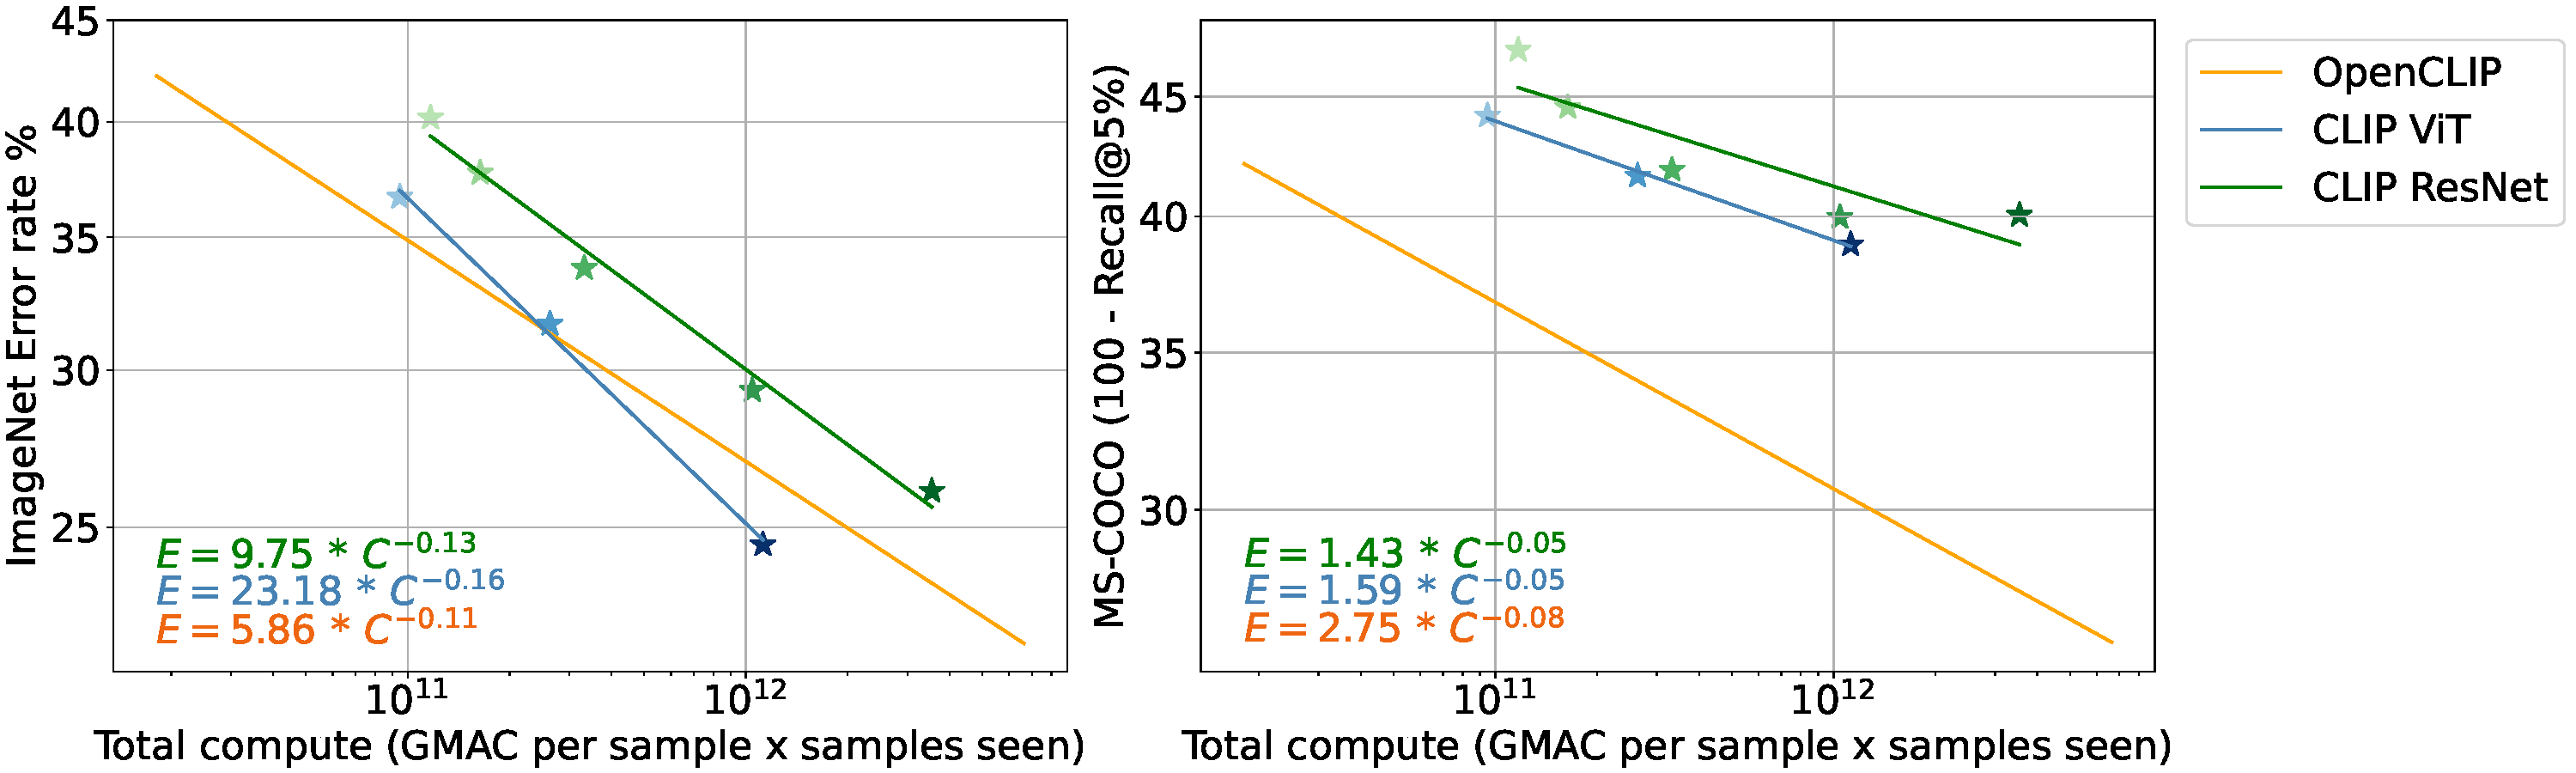
\includegraphics[width=\linewidth]{images/ViT_ResNet_openAI_openCLIP_zero-shot_ImageNet.pdf}
    \caption{Consistency of scaling trends for CLIP and openCLIP with additional CLIP ResNet models from OpenAI and trained on WIT. Relationship between total compute (GMAC) and ImageNet zero-shot classification error rate \textbf{(Left)} and with MS-COCO image retrieval at Recall@5 \textbf{(Right)}.}
    \label{fig:resnet_scaling_trends}
\end{figure*}

% \clearpage
\section{Code and Data availability}
\label{appendix:code}
We will provide source code used for running experiments and producing figures in this study at \url{https://github.com/LAION-AI/scaling-laws-openclip}. Links to pre-trained models obtained in this study and links to instructions for obtaining LAION-400m and LAION-5B used for pre-training experiments will be also made available there. All datasets used in the study are openly available and are listed together with references to the original work in Table \ref{tab:datasets_list}.


\begin{table}[!h]
\centering
\rowcolors{2}{light-light-gray}{white}
\begin{tabular}{@{}llll@{}}
%\begin{NiceTabular}{@{}llll@{}}
%\CodeBefore
%\rowcolors{2}{light-light-gray}{white}
%\Body
\toprule
\bf{Dataset} & \bf{Abbr.}  & \bf{Test size} & \bf{\#Classes}\\\midrule
ImageNet & INet & 50,000 &1,000\\
ImageNet-v2 & INet-v2 & 10,000 &1,000\\
ImageNet-R & INet-R & 30,000 &200\\
ImageNet Sketch & INet-S & 50,889 &1,000\\
ObjectNet & ObjNet & 18,574 &113\\
ImageNet-A & INet-A & 7,500 &200\\
CIFAR-10 & - & 10,000 &10\\
CIFAR-100 & - & 10,000 &100\\
MNIST & - & 10,000 &10\\
Oxford Flowers 102 & Flowers102 & 6,149 &102\\
Stanford Cars & Cars & 8,041 &196\\
SVHN & - & 26,032 &10\\
Facial Emotion Recognition 2013 & FER2013 & 7,178 &7\\
RenderedSST2 & - & 1,821 &2\\
Oxford-IIIT Pets & Pets & 3,669 &37\\
Caltech-101 & - & 6,085 &102\\
Pascal VOC 2007 Classification & VOC2007-Cl & 14,976 &20\\
SUN397 & - & 108,754 &397\\
FGVC Aircraft & - & 3,333 &100\\
Country211 & - & 21,100 &211\\
Describable Textures & DTD & 1,880 &47\\
GTSRB & - & 12,630 &43\\
STL10 & - & 8,000 &10\\
Diabetic Retinopathy & Retino & 42,670 &5\\
EuroSAT & - & 5,400 &10\\
RESISC45 & - & 6,300 &45\\
PatchCamelyon & PCAM & 32,768 &2\\
CLEVR Counts & - & 15,000 &8\\
CLEVR Object Distance & CLEVR Dist & 15,000 &6\\
DSPRITES Orientation & DSPRITES Orient & 73,728 &40\\
DSPRITES Position & DSPRITES pos & 73,728 &32\\
SmallNORB Elevation & SmallNORB Elv & 12,150 &9\\
SmallNORB Azimuth & SmallNORB Azim & 12,150 &18\\
DMLAB & - & 22,735 &6\\
KITTI closest vehicle distance & KITTI Dist & 711 &4\\ \midrule
%\midrule
%\multicolumn{2}{l}{Retrieval datasets} & & & \\
MS-COCO & - & 5,000 & -\\
Flickr30K & - & 1,000 & -\\
\bottomrule
%\end{NiceTabular}
\end{tabular}
\caption{Datasets used for evaluating downstream performance. Adapted from~\citep{Schuhmann2022}.}
\label{tab:datasets_list}
\end{table}

% Further details on the usage of the datasets in the conducted experiments are also provided in the repository linked above.
% \url{Link will be made available in final version}

% Only for final version
%\section*{Author Contributions}

% Only for final version
%\section*{Further Acknowledgements}

\section*{Broader and Social Impact}
\label{sec:impact}
% 
\textbf{Safety aspect.} Our work deals with studying function and properties of pre-trained models on large scales. Releasing these models to public can have both positive and negative implications, like with any research artefact that possesses generic functionality. We would like to stress that we consider the released pre-trained language-vision models as research artefacts that are there to advance the studies of scaling laws and allow analysis of the properties and behavior of such models for the broader research community. These models are not meant to be incorporated into end products or even used for applications in sensitive areas like interpretation of medical imaging in hospitals or security surveillance. There is potential for abuse of technology based on large-scale pre-trained generalist models, and it is the task of democratic institutions to work out rules for sensitive applications that might involve those. Open release of models gives the broad research community also opportunity to  study safety related aspects of such models, such to preventively design measures that make such abuse by malicious parties less probable, in a common transparent effort. Same applies to the common effort of studying yet not systematically understood biases that such models may contain due to pre-training on either largely uncurated, imbalanced data or on data filtered by models that already contain unknown biases (like OpenAI's CLIP that was trained on the private WIT-400M dataset), and due to the simplistic nature of the contrastive InfoNCE loss that drives learning.

\textbf{Energy cost.} There is high computational cost bound to pre-training experiments on large scale. Supercomputers used in our studies are highly ranked in the Green Top-500 list, ensuring that energy costs are dampened. In addition, strongly transferable pre-trained models save energy on numerous downstream tasks where they can perform in data-efficient and thus in an energy saving manner. Releasing such pre-trained models to public incurs additional energy savings, as research community can re-use already validated models without necessity to train those from scratch again.     


% Only for final version
\section*{Author Contributions}
\begin{itemize}
\item \textbf{Mehdi Cherti}: Planned and executed experiments on JUWELS Booster and Stability AI HPC, coordinated and performed results collection, distillation and analysis, performed deduplication analysis on LAION and downstream targest datasets, manuscript writing and revision.
\item \textbf{Romain Beaumont}: Planned and executed experiments on JUWELS Booster and Stability AI HPC, pioneered training of large scale openCLIP ViT H-14 and g-14, manuscript revision.
\item \textbf{Ross Wightman}: Planned and executed experiments on JUWELS Booster and Stability AI HPC, performed full fine-tuning experiments, manuscript writing and revision.
\item \textbf{Mitchell Wortsman}: experiment design and planning, performed experiments evaluating linear probing fine-tuning performance and robustness on ImageNet and other downstream datasets, manuscript writing and revision.
\item \textbf{Gabriel Ilharco}: experiment design and planning, performed experiments evaluating full fine-tuning performance and robustness on ImageNet and other downstream datasets, manuscript writing and revision.
\item \textbf{Cade Gordon}: implemented local contrastive loss for efficient distributed training, manuscript writing and revision.
\item \textbf{Christoph Schuhmann}: supervised larger scale experiments, resource and community organization, compute and storage resource acquisition, manuscript revision.
\item \textbf{Ludwig Schmidt}: provided advice on experiment design and study directions, manuscript writing and revision, general supervision
\item \textbf{Jenia Jitsev}: led the project; conducted experiments on various scales using JUWELS Booster and Stability AI HPC, scientific organization \& manuscript writing, ethical and social content, experiments planning and design, compute and storage resource acquisition, general supervision.

\end{itemize}


% Only for final version
% \section*{Acknowledgements}

\end{appendix}
